% !TEX program = pdflatex
%
% Permanent-magnet levitation project writeup.
% Compile with: pdflatex writeup.tex   (run twice for the table of contents)
%
\documentclass[11pt]{article}

\usepackage[a4paper,margin=1in]{geometry}
\usepackage{graphicx}
\usepackage{amsmath}
\usepackage{amssymb}
\usepackage{xcolor}
\usepackage{caption}
\usepackage{subcaption}
\usepackage{booktabs}
\usepackage{float}
\usepackage[hidelinks]{hyperref}

% --- look for figures in all the bundled subfolders by basename ---------------
\graphicspath{
  {./}
  {project_photos/}
  {graphs/test_charge/images/}
  {graphs/test_dipole/images/}
  {Attempt_3/}
  {Attempt_3/platform_optimizer/}
}

\captionsetup{font=small,labelfont=bf}

\title{\textbf{A Permanent-Magnet Levitating Platform:\\
Design, Simulation, and Why It Cannot Float}}
\author{Irakli Bakuradze}
\date{\today}

\begin{document}
\maketitle

\begin{abstract}
\noindent
The goal of this project was to build a platform that levitates in mid-air,
held up by nothing but permanent magnets: a fixed array of magnets on the
ground, repelling a second set of magnets on a free-floating platform. I
designed the magnet layout by hand, prototyped it with real neodymium magnets
on cardboard, modelled it in a physics simulation, and finally printed and
assembled a rigid version. The platform never floated
freely. This document records the build \emph{and} explains, with the
simulations as evidence, why the original goal is impossible for this method.
Two results do the explaining. First, \textbf{Earnshaw's theorem}: a body held
only by static inverse-square forces can never sit in a stable equilibrium, so
even a perfectly balanced platform must tip or slide away. Second, a less
well-known but equally fatal fact that the simulations uncovered directly: when
the vertical magnetic force is averaged over a \emph{plane} (which is exactly
what a flat platform does), the lift directly above each magnet is cancelled by
the attraction around it, and the net force tends to zero. The project
therefore ``failed'' in the sense of not levitating, but succeeded as an
investigation into why magnetic levitation is genuinely hard.
\end{abstract}

\tableofcontents
\bigskip

% =============================================================================
\section{Introduction and goal}
% =============================================================================

The objective was simple to state: \emph{make a platform that hovers above the
ground with no physical supports, using only permanent magnets}. The intended
mechanism is the most intuitive one imaginable -- put magnets on the floor with
their north poles facing up, put matching magnets under a platform with their
north poles facing down, and let like-poles-repel hold the platform aloft, the
way two repelling magnets pop apart in your hand.

Anyone who has tried this with two magnets knows the catch: the floating magnet
does not stay put. It squirts sideways and flips over. This project set out to
defeat that tendency by careful design -- many magnets, a clever layout, a wide
platform -- and to use simulation to find an arrangement that would be stable.
The headline result is that no such arrangement exists, and the value of the
work is in showing \emph{why}, both in theory and with the project's own data.

\paragraph{Outcome in one paragraph.} The platform did not levitate freely; the
best I achieved was a \emph{tethered} hover (Section~\ref{sec:build}), in which
a string or guide prevents the sideways/tip-over instability while the magnets
supply the lift. This is not a workmanship problem. It is forced by two
results that the rest of this document develops: Earnshaw's theorem
(Section~\ref{sec:earnshaw}) forbids a stable static equilibrium, and a
plane-averaging cancellation (Section~\ref{sec:lineplane}) means a flat
platform gets almost no \emph{net} lift to begin with.

% =============================================================================
\section{Physical principles}\label{sec:physics}
% =============================================================================

\subsection{The magnetic surface-charge model}

Throughout the project, magnets are modelled with the \emph{magnetic
surface-charge} (or ``Coulombian'') model. A uniformly magnetised block is
replaced by two charged faces: a $+$ pole face and a $-$ pole face carrying
surface charge density $\sigma_m = \pm M_0$. Each face is discretised into a
grid of point ``magnetic charges,'' and any two point charges $q_i,q_j$
interact through a Coulomb-like inverse-square law,
%
\begin{equation}
  \mathbf{F}_{ij} \;=\; \frac{\mu_0}{4\pi}\,
  \frac{q_i\,q_j}{\lvert \mathbf{r}_i-\mathbf{r}_j\rvert^{3}}\,
  (\mathbf{r}_i-\mathbf{r}_j).
  \label{eq:coulomb}
\end{equation}
%
The force between two magnets is the double sum of \eqref{eq:coulomb} over all
pole-charge pairs. This is more accurate than the simple point-dipole
approximation at the close range where levitation actually operates, while
still being cheap enough to evaluate millions of times inside an optimizer.
Because the model is linear, the force on a rigid assembly of magnets is just
the superposition of the single-magnet forces -- a fact the layout optimizer in
Section~\ref{sec:attempt3} exploits heavily.

\subsection{Two magnets: the dipole--dipole force}

A single magnet is the smallest interesting object: two opposite charges
separated by the magnet's thickness, i.e.\ a \emph{dipole}. The force one
magnet exerts on another is the dipole--dipole force, and its geometry is the
crux of everything that follows. Directly along the axis (one magnet stacked
above the other) like poles \emph{repel}; off to the sides the interaction
turns to \emph{attraction}. That sign change -- repulsion above, attraction
beside -- is not a detail, it is the reason flat platforms fail
(Section~\ref{sec:lineplane}).

\subsection{Earnshaw's theorem}\label{sec:earnshaw}

Earnshaw's theorem (1842) states that a collection of bodies interacting only
through inverse-square forces -- gravity, electrostatics, or magnetostatics
with fixed poles -- \emph{cannot rest in a stable static equilibrium}.

The proof is one line of vector calculus. In empty space the magnetic potential
energy $U$ of the platform obeys Laplace's equation,
%
\begin{equation}
  \nabla^2 U \;=\;
  \frac{\partial^2 U}{\partial x^2}
  + \frac{\partial^2 U}{\partial y^2}
  + \frac{\partial^2 U}{\partial z^2} \;=\; 0 .
  \label{eq:laplace}
\end{equation}
%
A \emph{stable} equilibrium requires $U$ to be a local minimum: a small
displacement in \emph{any} direction must raise the energy, so all three second
derivatives in \eqref{eq:laplace} must be positive. But \eqref{eq:laplace} says
they sum to zero. They cannot all be positive. The best one can do is a saddle:
stable along some axes, unstable along the rest. Concretely, if the platform is
stable vertically (it rises when pushed down and sinks when pushed up, balancing
gravity at one height), it is necessarily \emph{unstable} horizontally -- the
slightest sideways nudge or tilt grows, and it slides off or flips.

This is exactly the configuration this project tried to build, so the goal was
impossible from the start. The standard ways real systems escape Earnshaw are
all things this design deliberately does \emph{not} have:
%
\begin{itemize}
  \item \textbf{Diamagnets or superconductors} ($\mu<1$): pyrolytic graphite
        over magnets, or flux-pinned superconductors. These violate the
        assumptions of the theorem and \emph{can} levitate statically.
  \item \textbf{Spin stabilisation}: the Levitron top spins fast enough that
        gyroscopic precession converts the tip-over instability into a slow,
        bounded wobble.
  \item \textbf{Active feedback}: an electromagnet plus a position sensor
        constantly corrects the unstable axis (this is how maglev trains and
        magnetic bearings work).
  \item \textbf{Motion / eddy currents}: a moving conductor in a changing field
        generates stabilising induced currents.
\end{itemize}
%
A static array of permanent magnets is none of these, so it cannot win.

% =============================================================================
\section{Feasibility study by simulation}\label{sec:sim}
% =============================================================================

Before building anything I used simulation purely to check feasibility: ``is
there \emph{any} sense in which this floats?'' The force-field figures below
(generated with \texttt{numpy}/\texttt{matplotlib}; full descriptions in
\texttt{graphs/description\_of\_graphs.md}) build up the picture in two stages:
first the force on a single magnetic \emph{charge} near a magnet, then the force
on a whole \emph{magnet} (a dipole), which is the levitation-relevant case.

\subsection{Force on a test charge near a magnet}

Figure~\ref{fig:charge-fields} shows the force on a single $+$ test charge,
first for a point-dipole source (two charges) and then for a ``flat magnet''
source (two uniformly charged line segments). The arrows give force direction,
colour gives magnitude. Far from the magnet the flat magnet looks just like the
point dipole; close in it looks like two charged sheets.

\begin{figure}[H]
  \centering
  \begin{subfigure}{0.48\linewidth}
    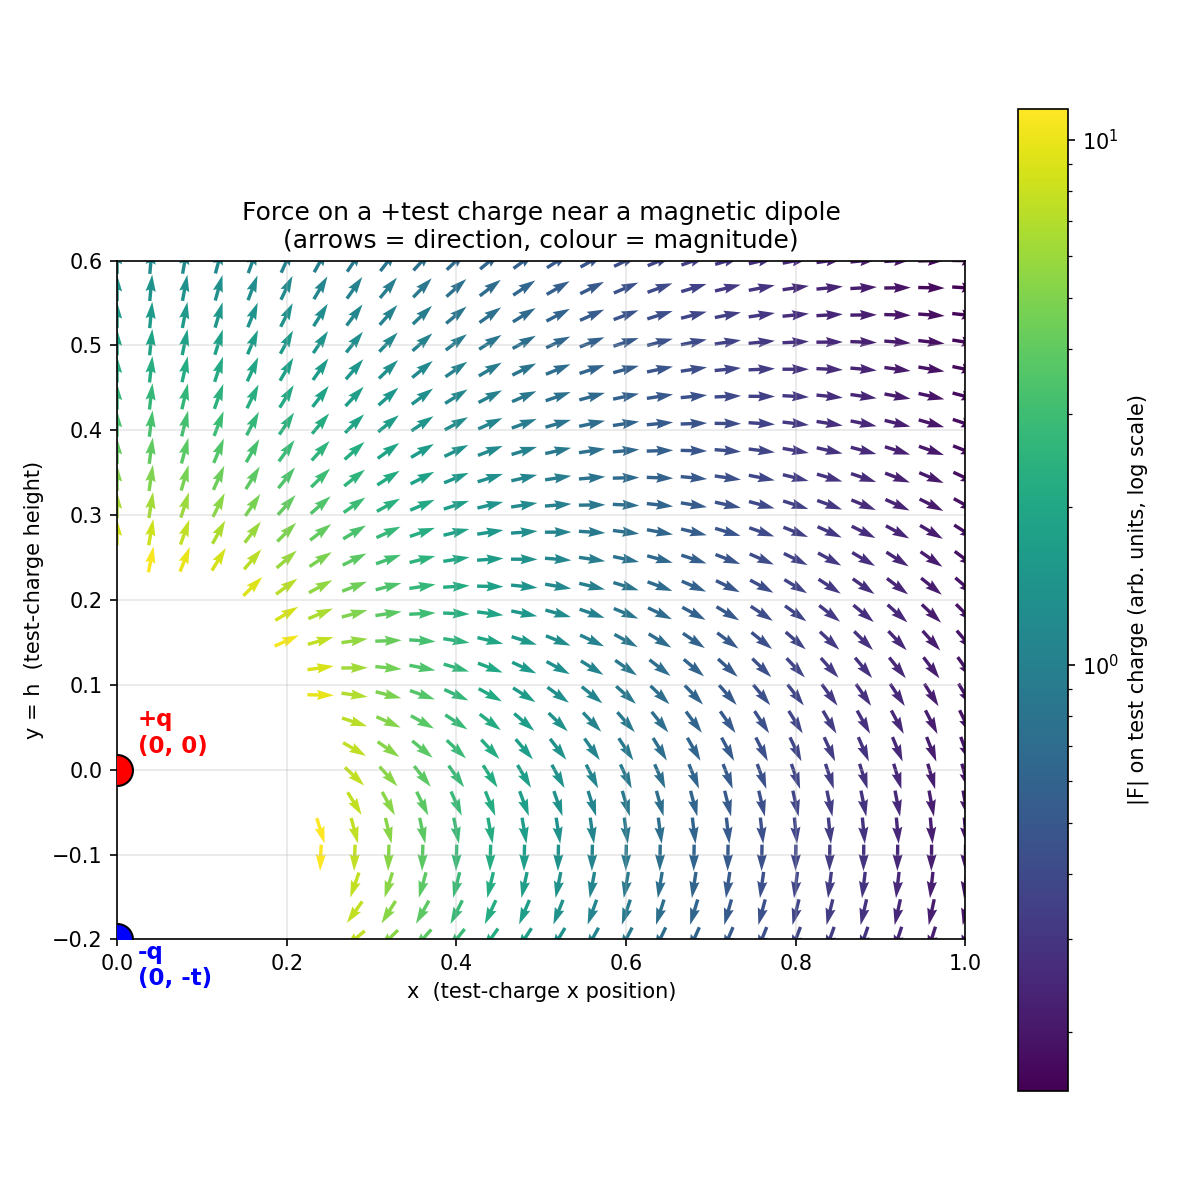
\includegraphics[width=\linewidth]{magnetic_dipole_force_field.png}
    \caption{Point-dipole source ($+q$ over $-q$).}
  \end{subfigure}\hfill
  \begin{subfigure}{0.48\linewidth}
    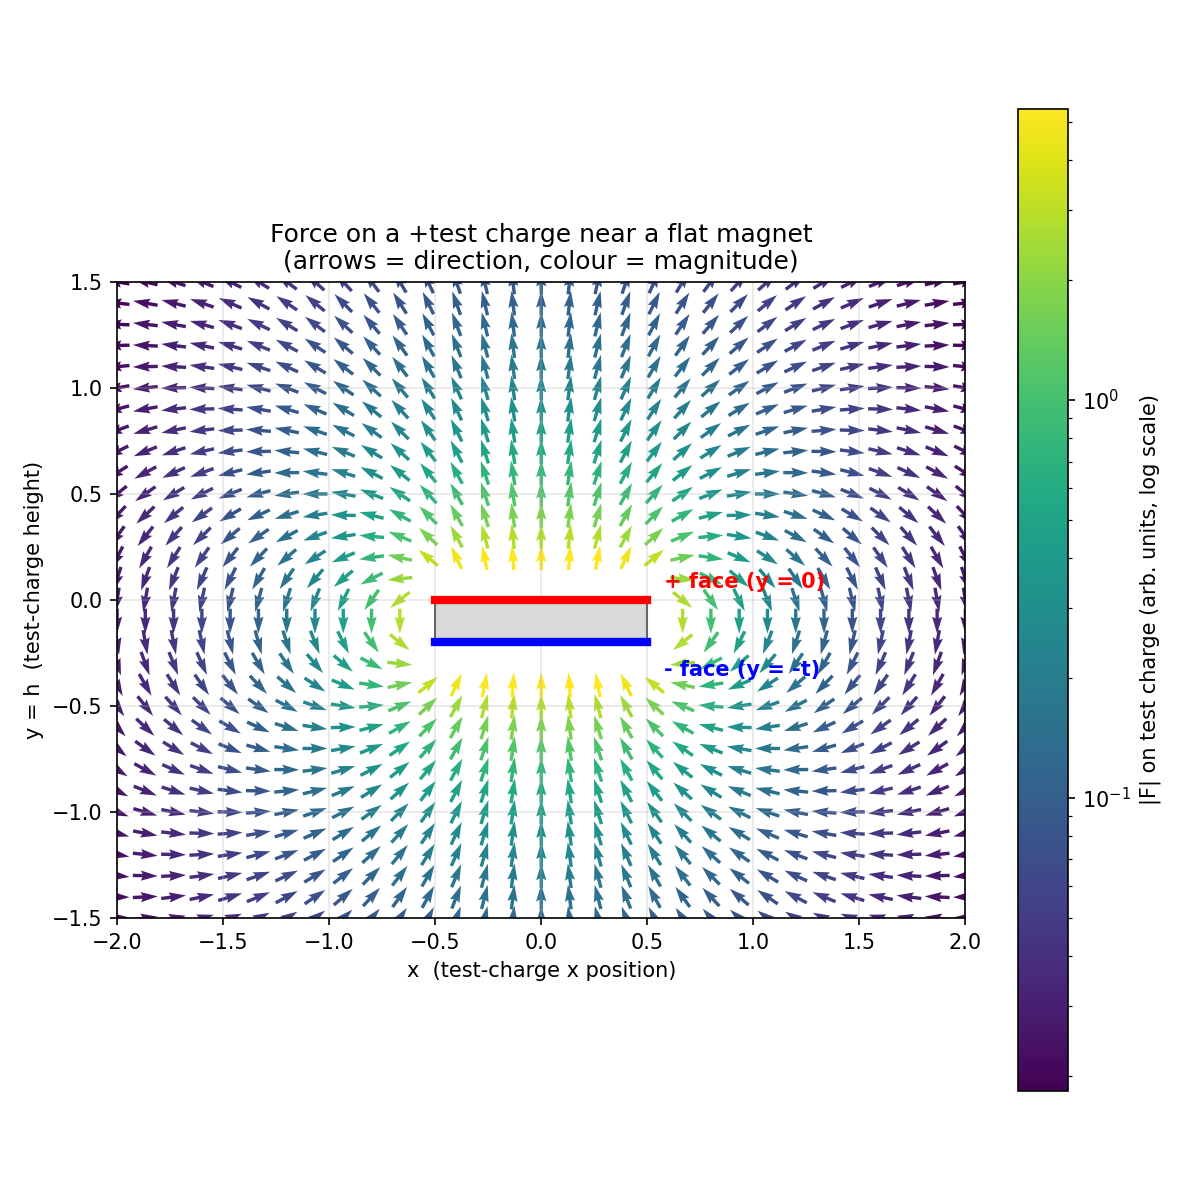
\includegraphics[width=\linewidth]{flat_magnet_force_field.png}
    \caption{Flat-magnet source (charged line segments).}
  \end{subfigure}
  \caption{Force on a positive test charge near a magnet. Red dot/line $=+$
  pole, blue $=-$ pole; arrows are force direction, colour is $\lvert
  \mathbf{F}\rvert$ (log scale).}
  \label{fig:charge-fields}
\end{figure}

\subsection{The lift component and the ``magic angle''}

Splitting out only the vertical component $F_y$ (the lift) makes the sign
structure visible: red where the force is up, blue where it is down
(Figure~\ref{fig:charge-fy}). The dashed curve is the $F_y=0$ locus separating
lift from pull-down. On the symmetric-log scale the zero curve far from the
magnet approaches the classic dipole \emph{magic-angle} lines $y = x/\sqrt2$:
the $3\cos^2\alpha - 1 = 0$ result at $\alpha \approx 54.7^\circ$ from the
dipole axis. The practical message is already here: the lift region is a narrow
cone directly above the pole, surrounded by pull-down everywhere else.

\begin{figure}[H]
  \centering
  \begin{subfigure}{0.48\linewidth}
    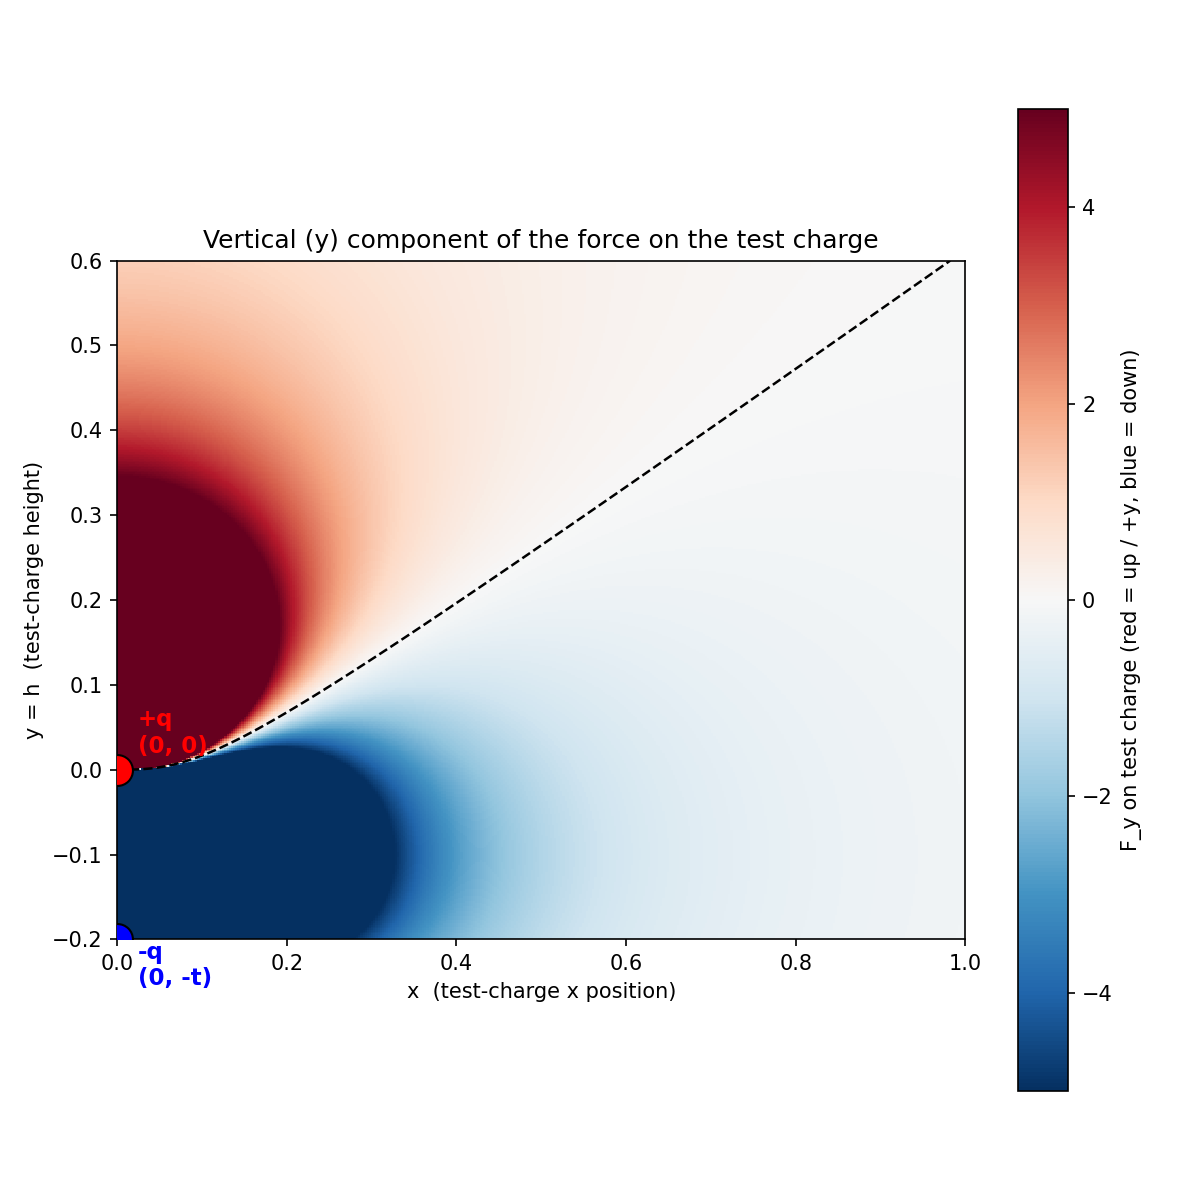
\includegraphics[width=\linewidth]{magnetic_dipole_force_Fy.png}
    \caption{$F_y$, linear scale (red up, blue down).}
  \end{subfigure}\hfill
  \begin{subfigure}{0.48\linewidth}
    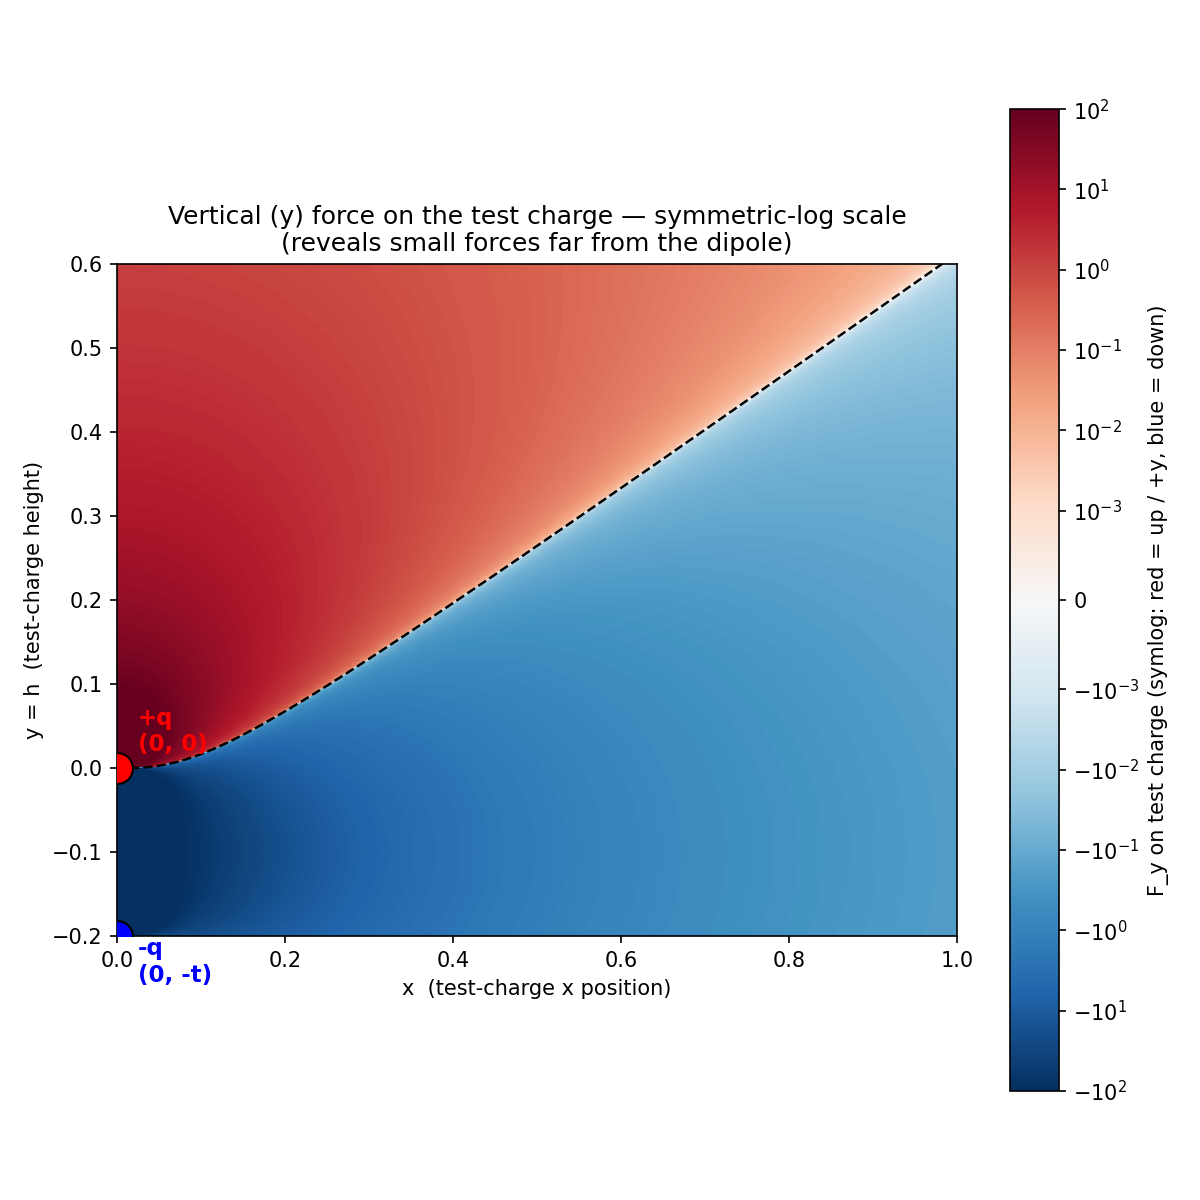
\includegraphics[width=\linewidth]{magnetic_dipole_force_Fy_symlog.png}
    \caption{$F_y$, symmetric-log scale; zero curve $\to$ magic-angle lines.}
  \end{subfigure}
  \caption{Vertical force component for the point-dipole source. The dashed
  curve is $F_y=0$.}
  \label{fig:charge-fy}
\end{figure}

\subsection{Force on a test \emph{magnet} (the real case)}

The levitation-relevant object is a magnet floating above a magnet, so the test
object is itself a dipole. With the floating magnet \emph{flipped} (its $+$ pole
facing the source's $+$ pole), the column directly above the source is
repulsive -- this is the levitation configuration. Figure~\ref{fig:dipole}
shows the net force field and its vertical component: a red (upward) column
straight above the source, flanked by blue (downward/attractive) regions, just
as the single-charge picture predicted.

\begin{figure}[H]
  \centering
  \begin{subfigure}{0.48\linewidth}
    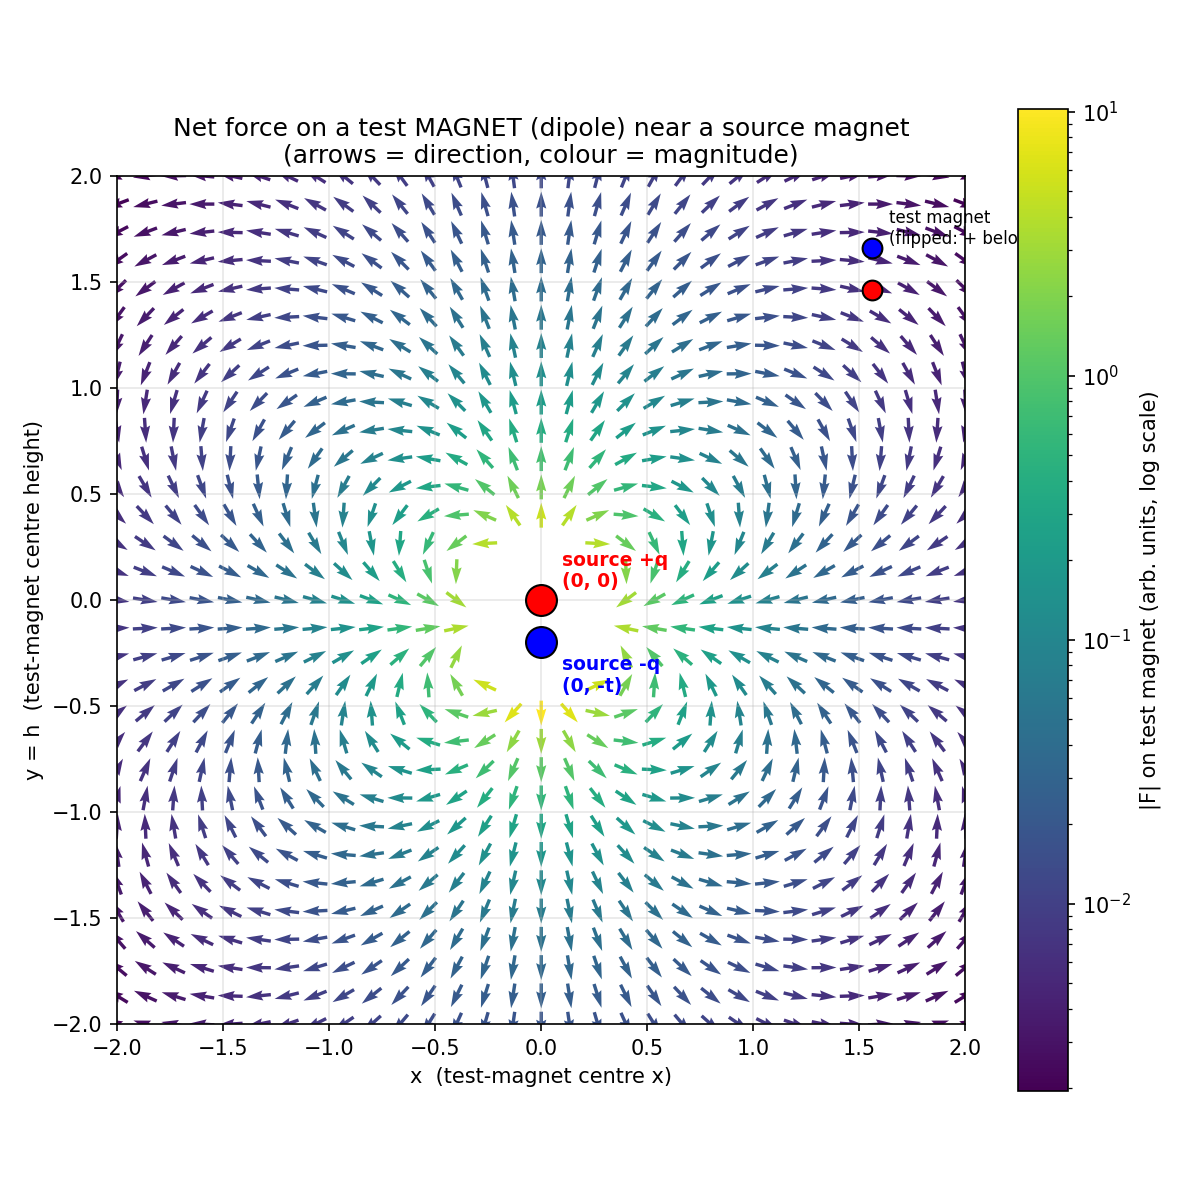
\includegraphics[width=\linewidth]{dipole_dipole_force_field.png}
    \caption{Net force on the flipped test magnet.}
  \end{subfigure}\hfill
  \begin{subfigure}{0.48\linewidth}
    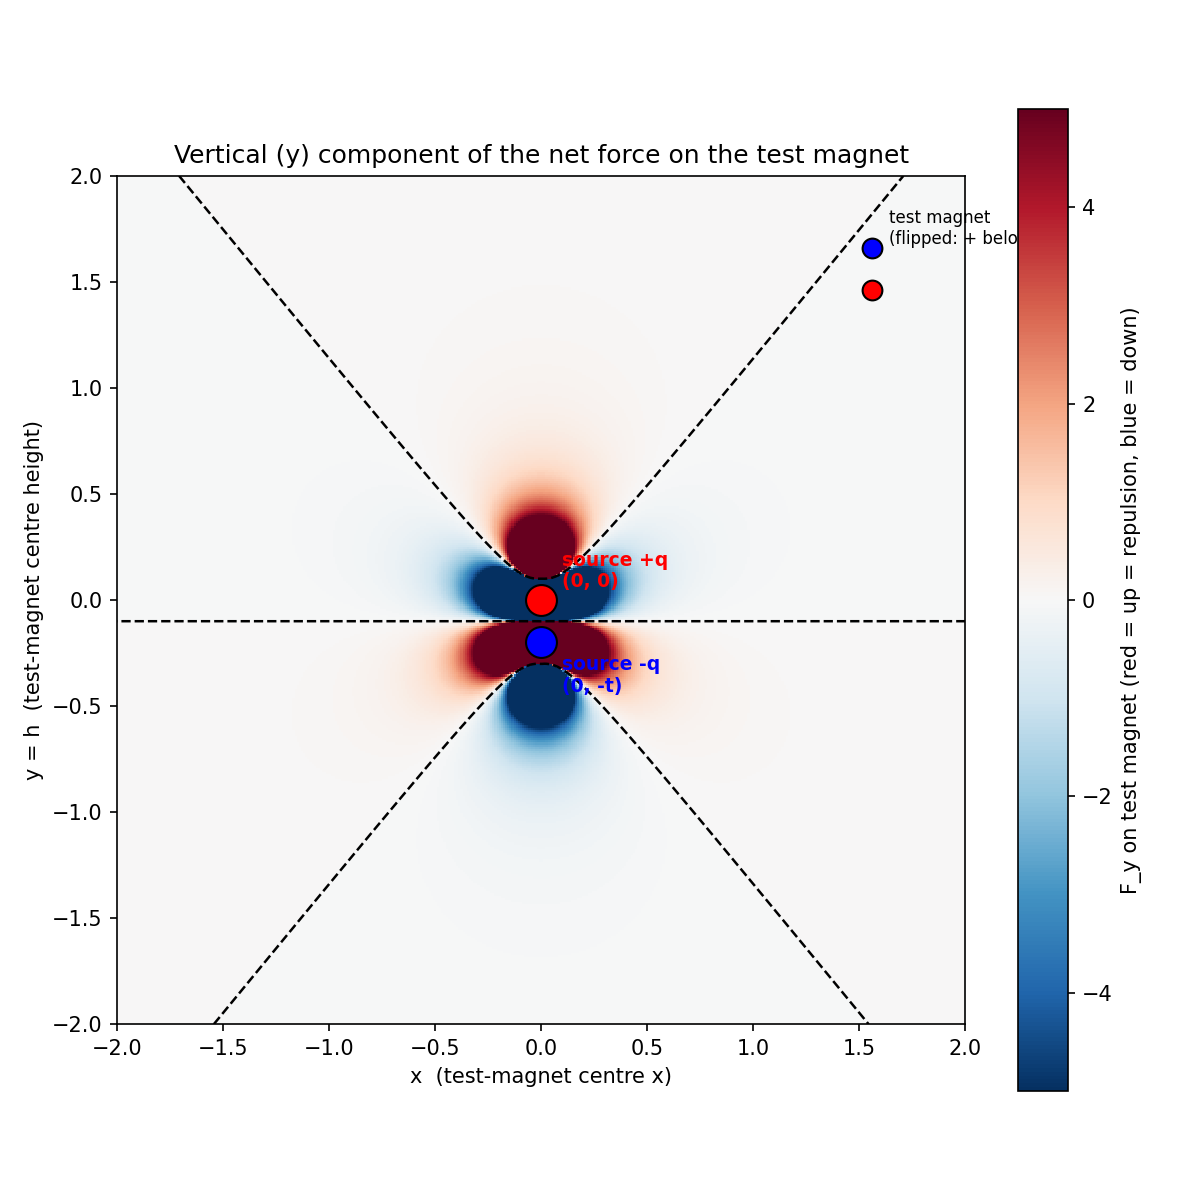
\includegraphics[width=\linewidth]{dipole_dipole_force_Fy.png}
    \caption{Vertical component: red column = lift above the source.}
  \end{subfigure}
  \caption{Magnet-on-magnet (dipole--dipole) force. Directly above: repulsion
  (lift). To the sides: attraction. This sign pattern is the seed of the
  cancellation in Section~\ref{sec:lineplane}.}
  \label{fig:dipole}
\end{figure}

% =============================================================================
\section{Why a flat platform gets almost no lift}\label{sec:lineplane}
% =============================================================================

This is the most important -- and least obvious -- result of the project, and
it is separate from Earnshaw. Earnshaw says the platform cannot be
\emph{stable}. This section says a wide flat platform barely gets any net
\emph{lift} in the first place.

Look again at the vertical-force field of one magnet
(Figure~\ref{fig:dipole}b): a positive (up) core directly above the pole,
surrounded by a negative (down) ring. Now ask what a platform feels. A platform
is a sheet of magnets spread over an \emph{area}, so the net vertical force is
the field summed over that area. The decisive comparison is between integrating
the field along a \emph{line} versus over a \emph{plane}:
%
\begin{equation}
  I_{\text{line}}(s) = \int_{-s}^{s} F_z(x,0)\,dx,
  \qquad
  I_{\text{plane}}(R) = \iint_{x^2+y^2 \le R^2} F_z\, dA .
  \label{eq:lineplane}
\end{equation}
%
For the dipole--dipole kernel these have closed-form limits. The line integral
tends to a nonzero value ($\approx +0.83$ in the script's units), but the plane
integral tends to \textbf{zero}:
%
\begin{equation}
  I_{\text{plane}}(\infty) = \sum_{\text{pole pairs}} 2\pi\,(\text{sign})
  = 2\pi(+1-1-1+1) = 0 .
\end{equation}
%
The positive lift above each magnet is \emph{exactly} cancelled by the
attractive ring around it. This is a direct consequence of there being no
magnetic monopoles ($\nabla\cdot\mathbf{B}=0$): the vertical force, averaged
over a plane, has to vanish. Figure~\ref{fig:lineplane} shows the two
accumulations side by side -- the line integral saturates at a healthy positive
value while the plane integral climbs, then collapses back to zero.

\begin{figure}[H]
  \centering
  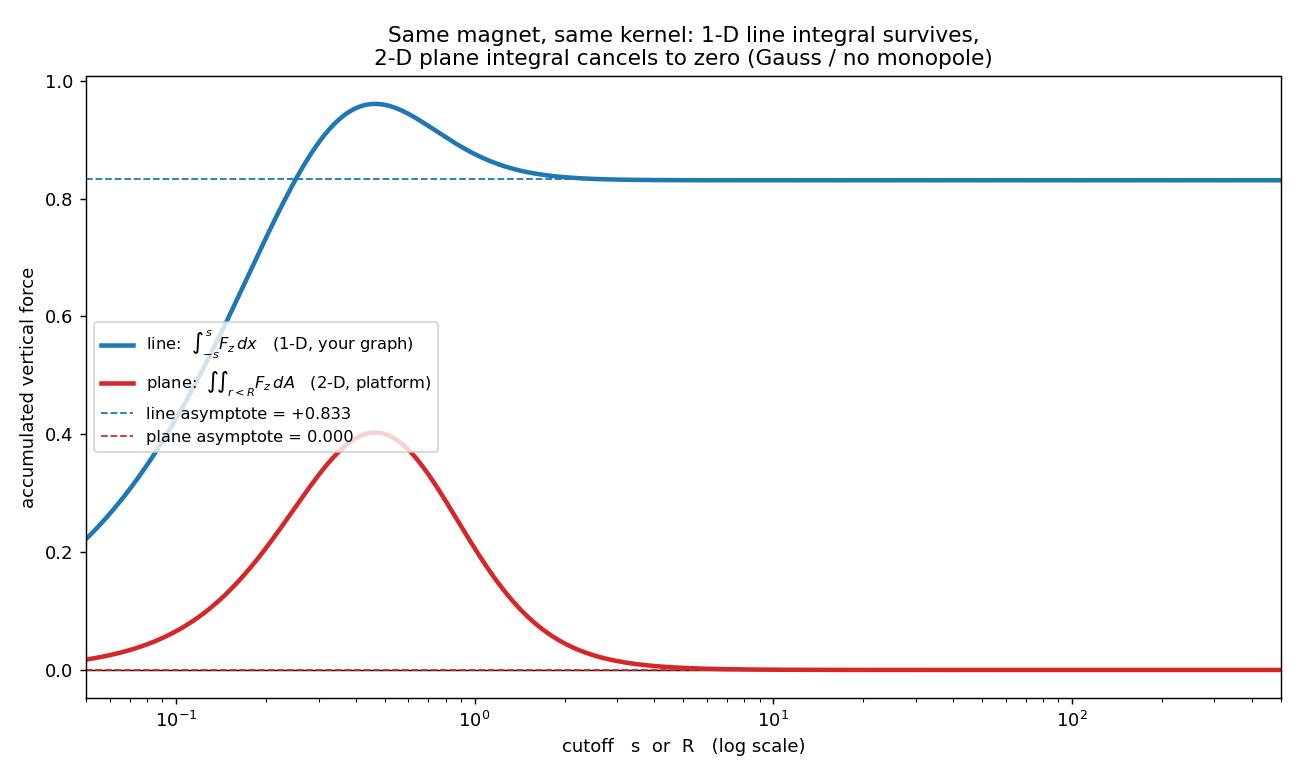
\includegraphics[width=0.8\linewidth]{line_vs_plane.png}
  \caption{Same magnet, same force law: the 1-D \emph{line} integral of $F_z$
  saturates at a nonzero value (blue), but the 2-D \emph{plane} integral
  cancels to zero (red). Looking at a single slice makes levitation look
  feasible; spreading magnets over an area makes the net lift vanish.}
  \label{fig:lineplane}
\end{figure}

\paragraph{Consequence.} The wider and flatter you make the platform -- the very
thing intuition says should help -- the closer the average lift per magnet
drives toward zero. \emph{This is the answer to ``why is the force so low.''} It
is not a tuning failure; the optimizer of Section~\ref{sec:attempt3} was trying
to push up a quantity whose spatial average is structurally near zero.

% =============================================================================
\section{Worst-case layout optimization}\label{sec:attempt3}
% =============================================================================

With the feasibility settled, the central simulation asked a sharper question:
\emph{given a fixed rectangular ground array, what arrangement of platform
magnets maximises the lift even in the worst landing position?} The platform
carries $N$ magnets at planar offsets
$\{\mathbf{r}_i\}$; dropped onto the array at a random translation $T$ and
rotation $\theta$, its net vertical force is, by superposition,
%
\begin{equation}
  F_z(T,\theta) \;=\; \sum_{i=1}^{N} F_z^{\text{single}}\!\big(R(\theta)\,\mathbf{r}_i + T\big),
\end{equation}
%
where $F_z^{\text{single}}$ is the precomputed single-magnet field. I drew many
random placements, took the \emph{worst} $15\%$ by vertical force (a
conditional-value-at-risk objective), and ran gradient \emph{ascent} (Adam) on
the magnet offsets to lift that worst tail:
%
\begin{equation}
  \max_{\{\mathbf{r}_i\}} \;\; \frac{1}{k}\!\!\sum_{\text{worst }15\%}\!\! F_z(T,\theta),
  \qquad k = \lceil 0.15\,N_{\text{samples}}\rceil .
\end{equation}
%
The field is sampled by bilinear interpolation, so the gradient of the objective
with respect to each magnet offset is available analytically (chained through
the rotation $R(\theta)$). Optimizing the worst tail rather than the mean
directly targets stability: it is the bad landings that make a platform crash.

\begin{figure}[H]
  \centering
  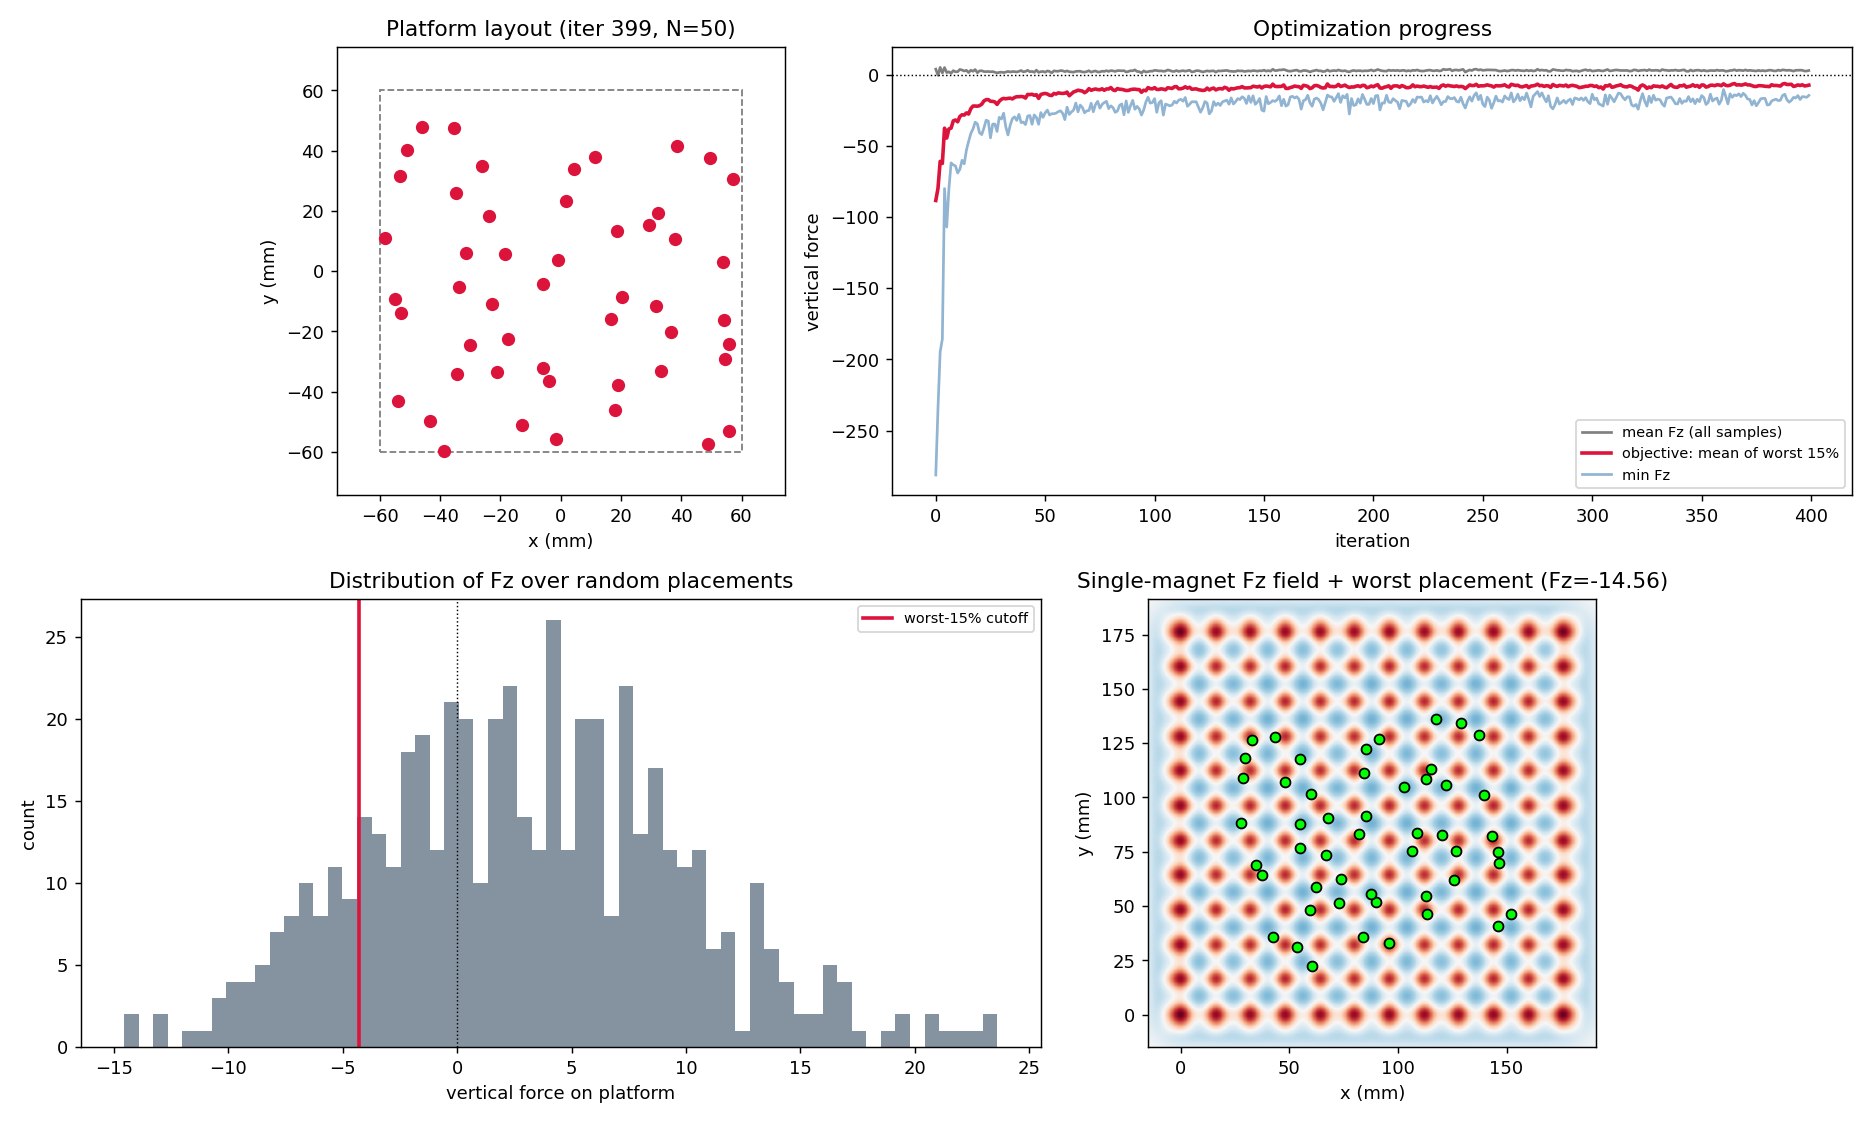
\includegraphics[width=\linewidth]{optimization_result.png}
  \caption{Live optimizer dashboard. Top-left: evolving platform layout.
  Top-right: learning curve -- mean $F_z$ (grey), the worst-$15\%$ objective
  (crimson), and the minimum (blue). Bottom-left: distribution of net $F_z$ over
  random placements. Bottom-right: the single-magnet $F_z$ field with the
  current worst placement overlaid.}
  \label{fig:optresult}
\end{figure}

\paragraph{What the optimizer revealed.} Even after optimization the worst-case
vertical force stays stubbornly small, and a significant fraction of placements
remain \emph{negative} (net downward). The diagnostic figure
(Figure~\ref{fig:diagnosis}) shows why, and ties straight back to
Section~\ref{sec:lineplane}: the single-magnet vertical force is positive
directly over a magnet but negative in the gaps (left panel), so the net force on
the platform is a near-cancellation whose mean is barely positive with a fat
negative tail (right panel). The optimizer is fighting a quantity whose plane
average is essentially zero; no layout can change that.

\begin{figure}[H]
  \centering
  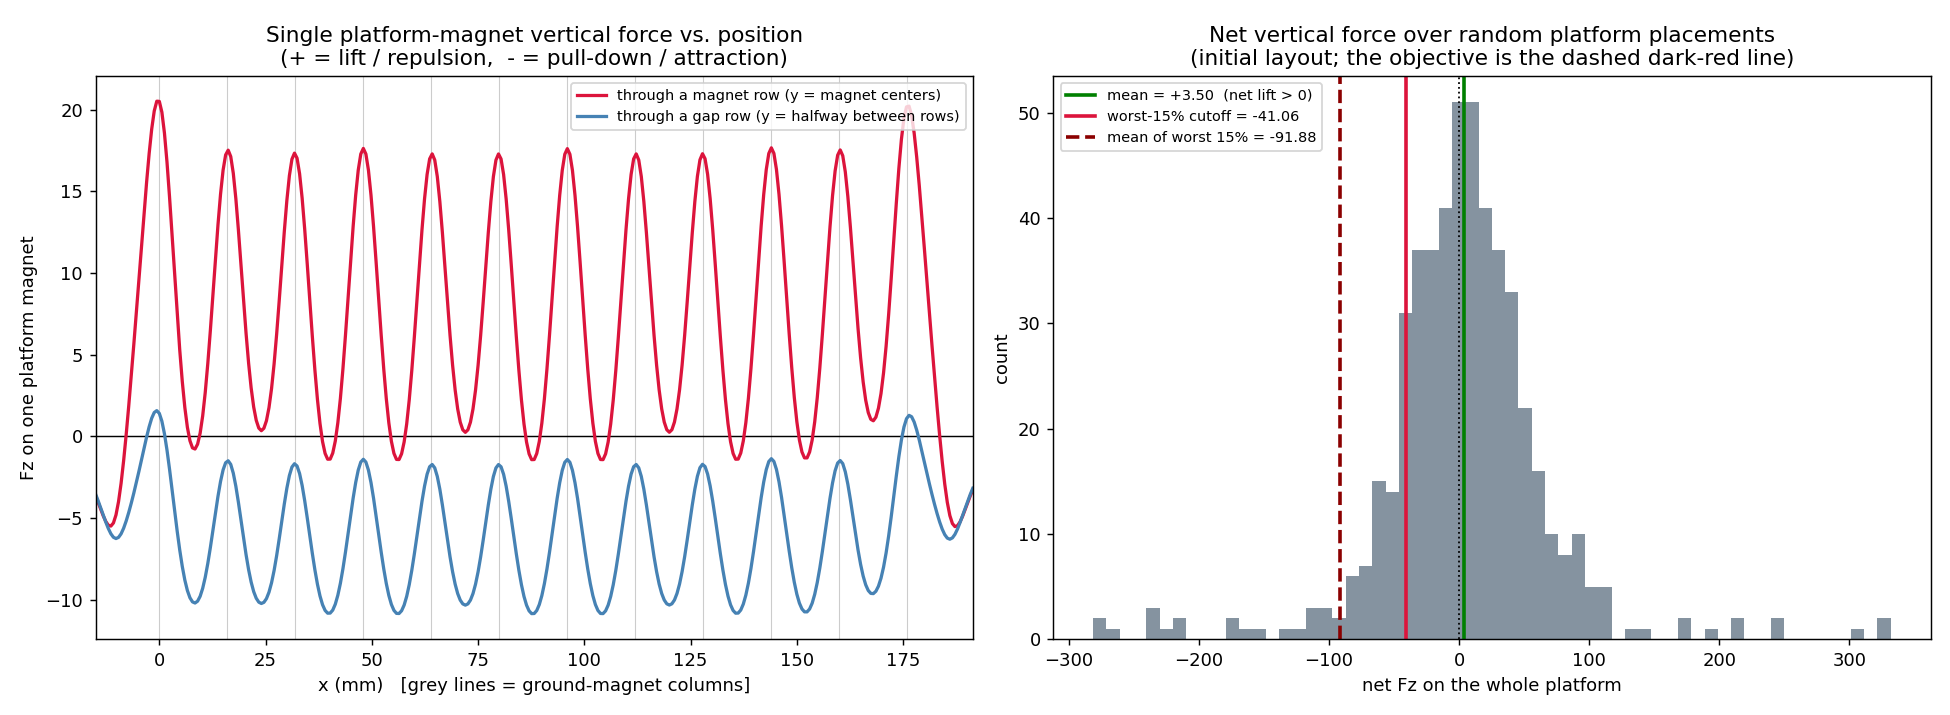
\includegraphics[width=\linewidth]{diagnosis.png}
  \caption{Left: horizontal slices of the single-magnet $F_z$ field -- positive
  (lift) over magnet rows, negative (pull-down) over the gaps. Right:
  distribution of net $F_z$ over random platform placements; the mean is only
  just positive and the worst-$15\%$ tail is negative -- placements that would
  crash.}
  \label{fig:diagnosis}
\end{figure}

\begin{table}[H]
  \centering
  \caption{Key simulation parameters (layout optimizer).}
  \begin{tabular}{ll}
    \toprule
    Parameter & Value \\
    \midrule
    Ground magnet (model)      & $10 \times 10 \times 2$ mm block \\
    Ground array               & $12 \times 12$, $16$ mm spacing \\
    Platform magnets           & $50$, clamped within $120\times120$ mm \\
    Hover gap $h$              & $4$ mm \\
    Samples per iteration      & $512$ random $(T,\theta)$ \\
    Worst-case fraction        & $15\%$ (CVaR) \\
    Iterations                 & $400$, Adam, lr $0.5$ \\
    \bottomrule
  \end{tabular}
  \label{tab:params}
\end{table}

% =============================================================================
\section{Physical construction}\label{sec:build}
% =============================================================================

In parallel with the simulations I built the thing, both to develop intuition
and to document the attempt.

\subsection{Planning the layout by hand}

I began on cardboard, sketching candidate magnet positions and using the drawing
to reason about the resulting field. In these diagrams \textbf{black marks a
north pole and red marks a south pole}. Figure~\ref{fig:sketches} shows the
progression: a bare position sketch, then the same layout annotated with the
field and a single ``test'' magnet placed at the centre.

This is where the first surprise appeared. I had laid out every magnet with its
\emph{north} pole facing up, expecting a uniform field of north poles and hence
repulsion everywhere. Instead, drawing out the field showed \emph{south} poles
emerging in the gaps \emph{between} the magnets (the red regions): because the
magnets were not packed closely enough, the field lines looping from one
magnet's north pole to its own south pole curve back through the gaps, so a
small magnet sitting between two ground magnets sees an effective south pole and
is \emph{attracted} downward rather than repelled. The intended ``all
repulsion'' surface was really repulsion over each magnet separated by
attraction in the gaps -- the same up-over-the-pole, down-in-the-gap pattern the
simulation predicts (Figure~\ref{fig:diagnosis}).

\begin{figure}[H]
  \centering
  \begin{subfigure}{0.31\linewidth}
    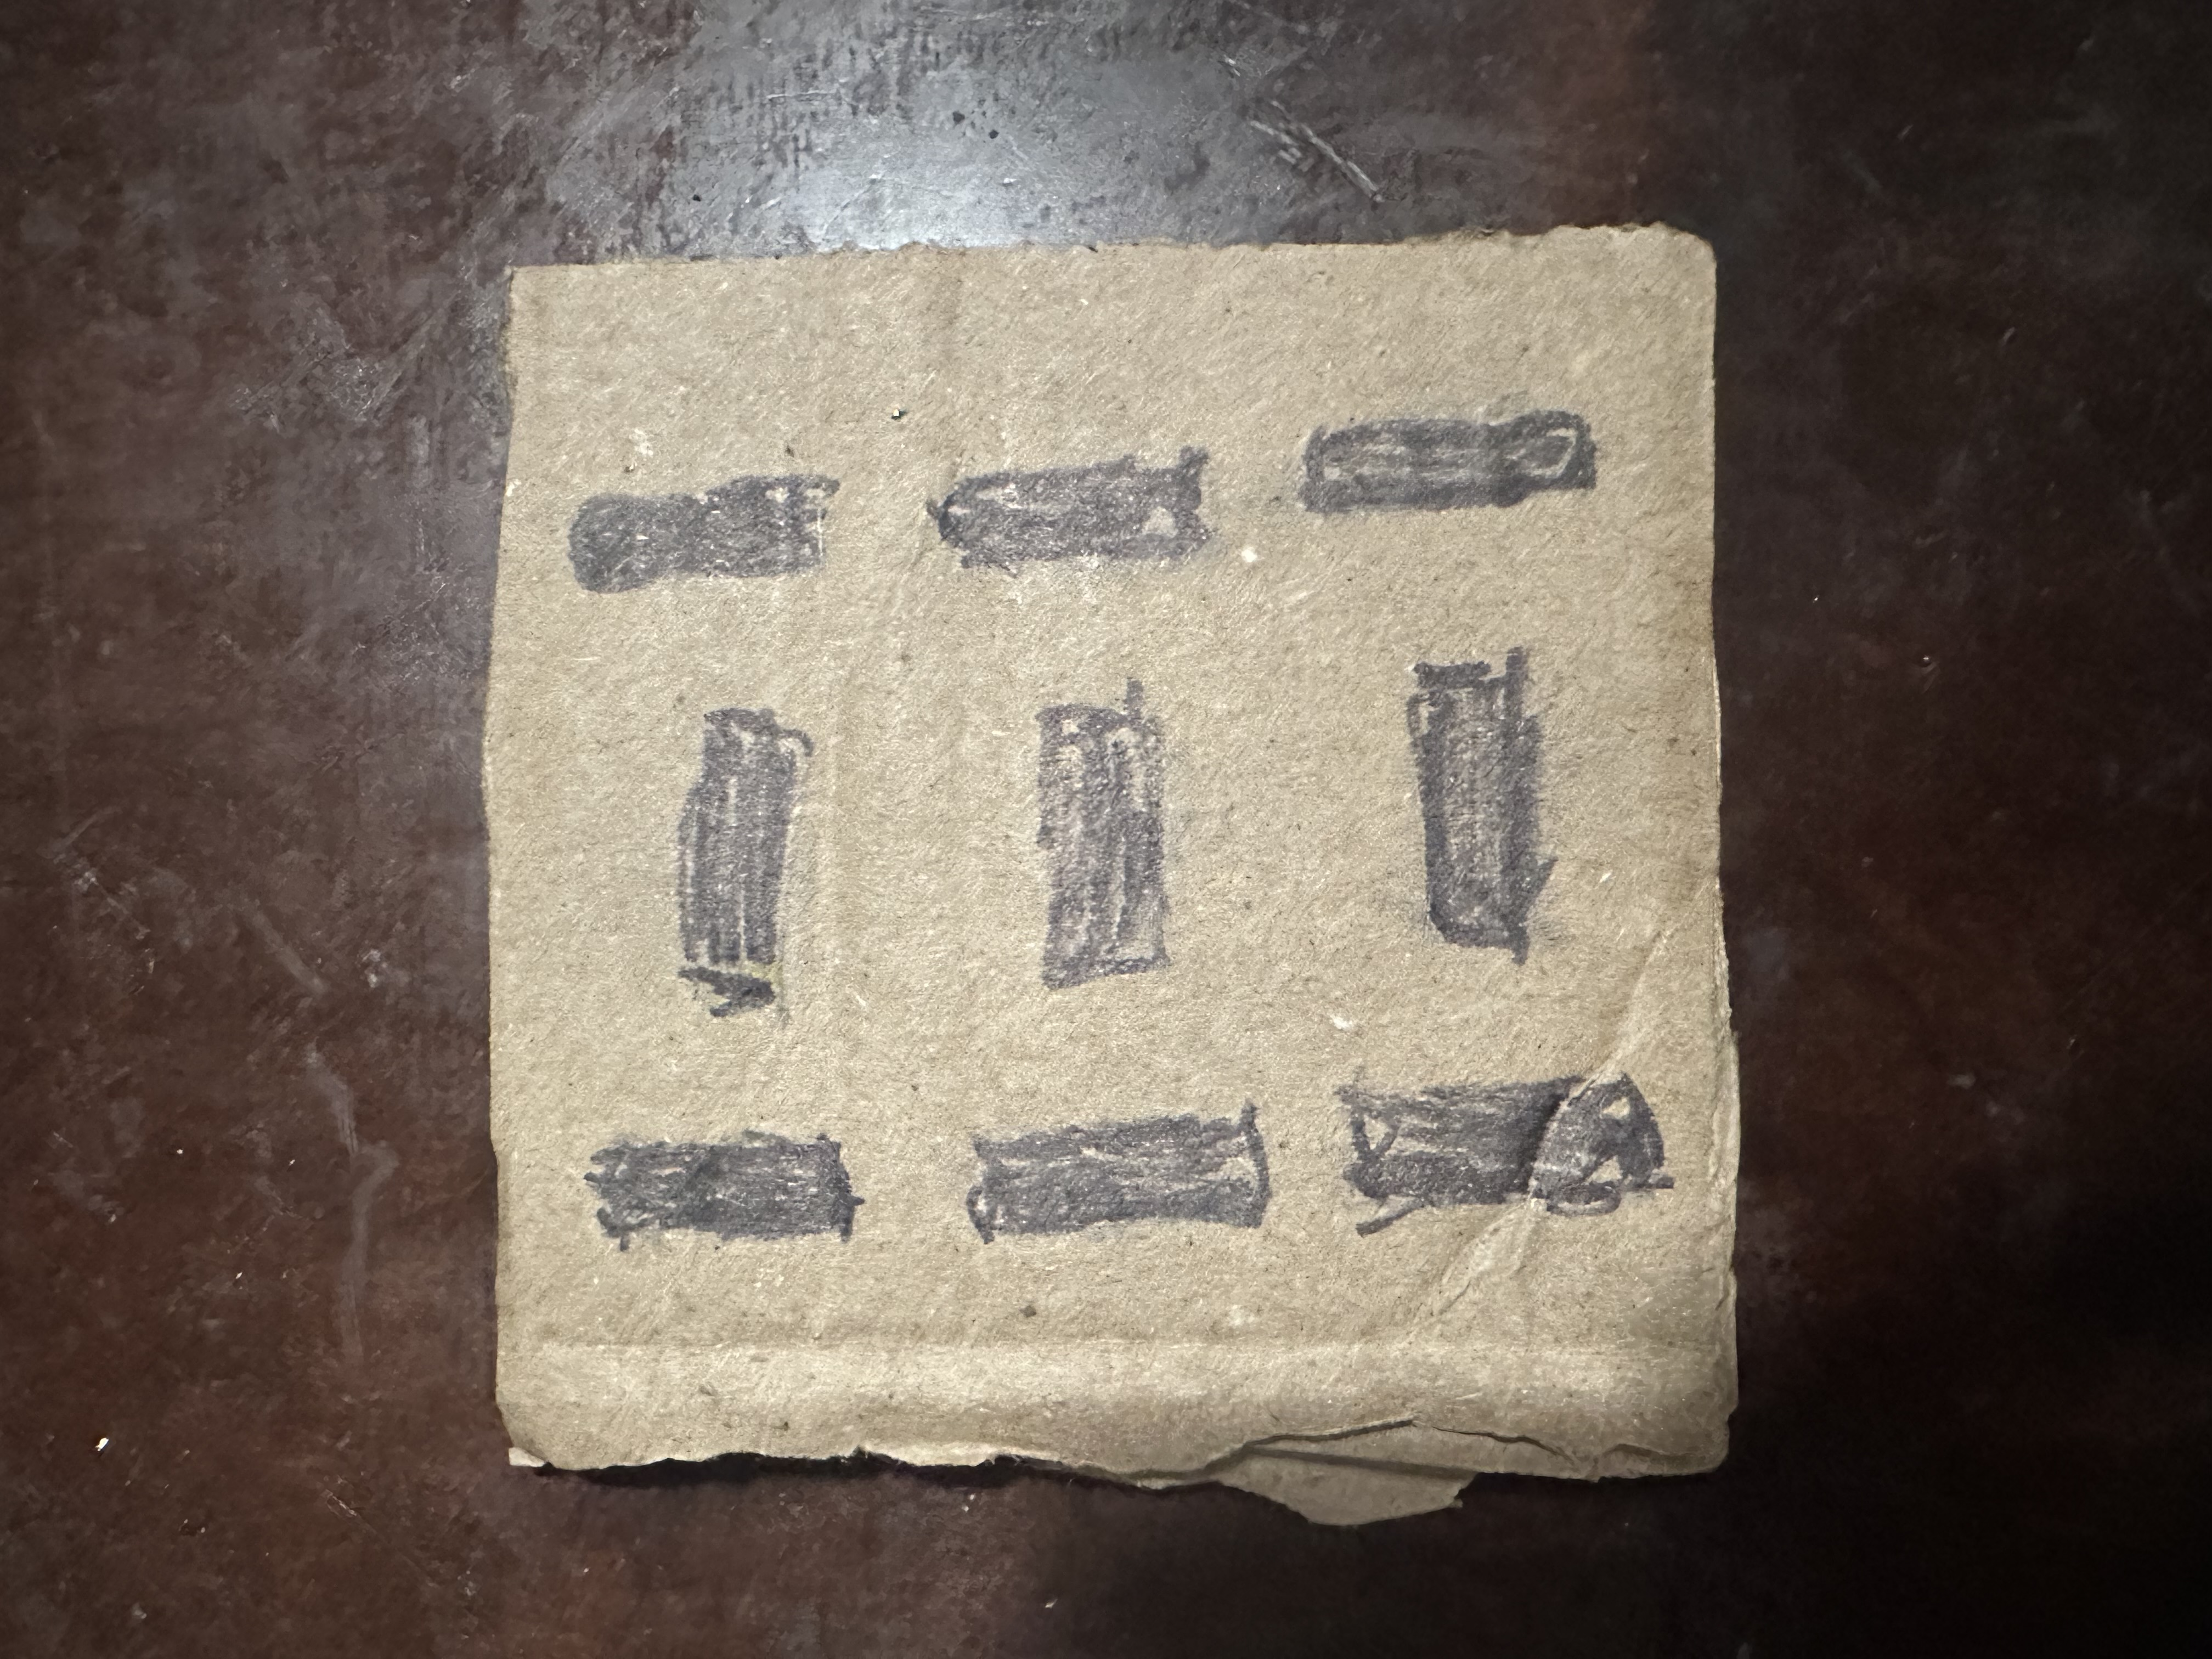
\includegraphics[width=\linewidth]{IMG_0335.jpeg}
    \caption{Bare position sketch.}
  \end{subfigure}\hfill
  \begin{subfigure}{0.31\linewidth}
    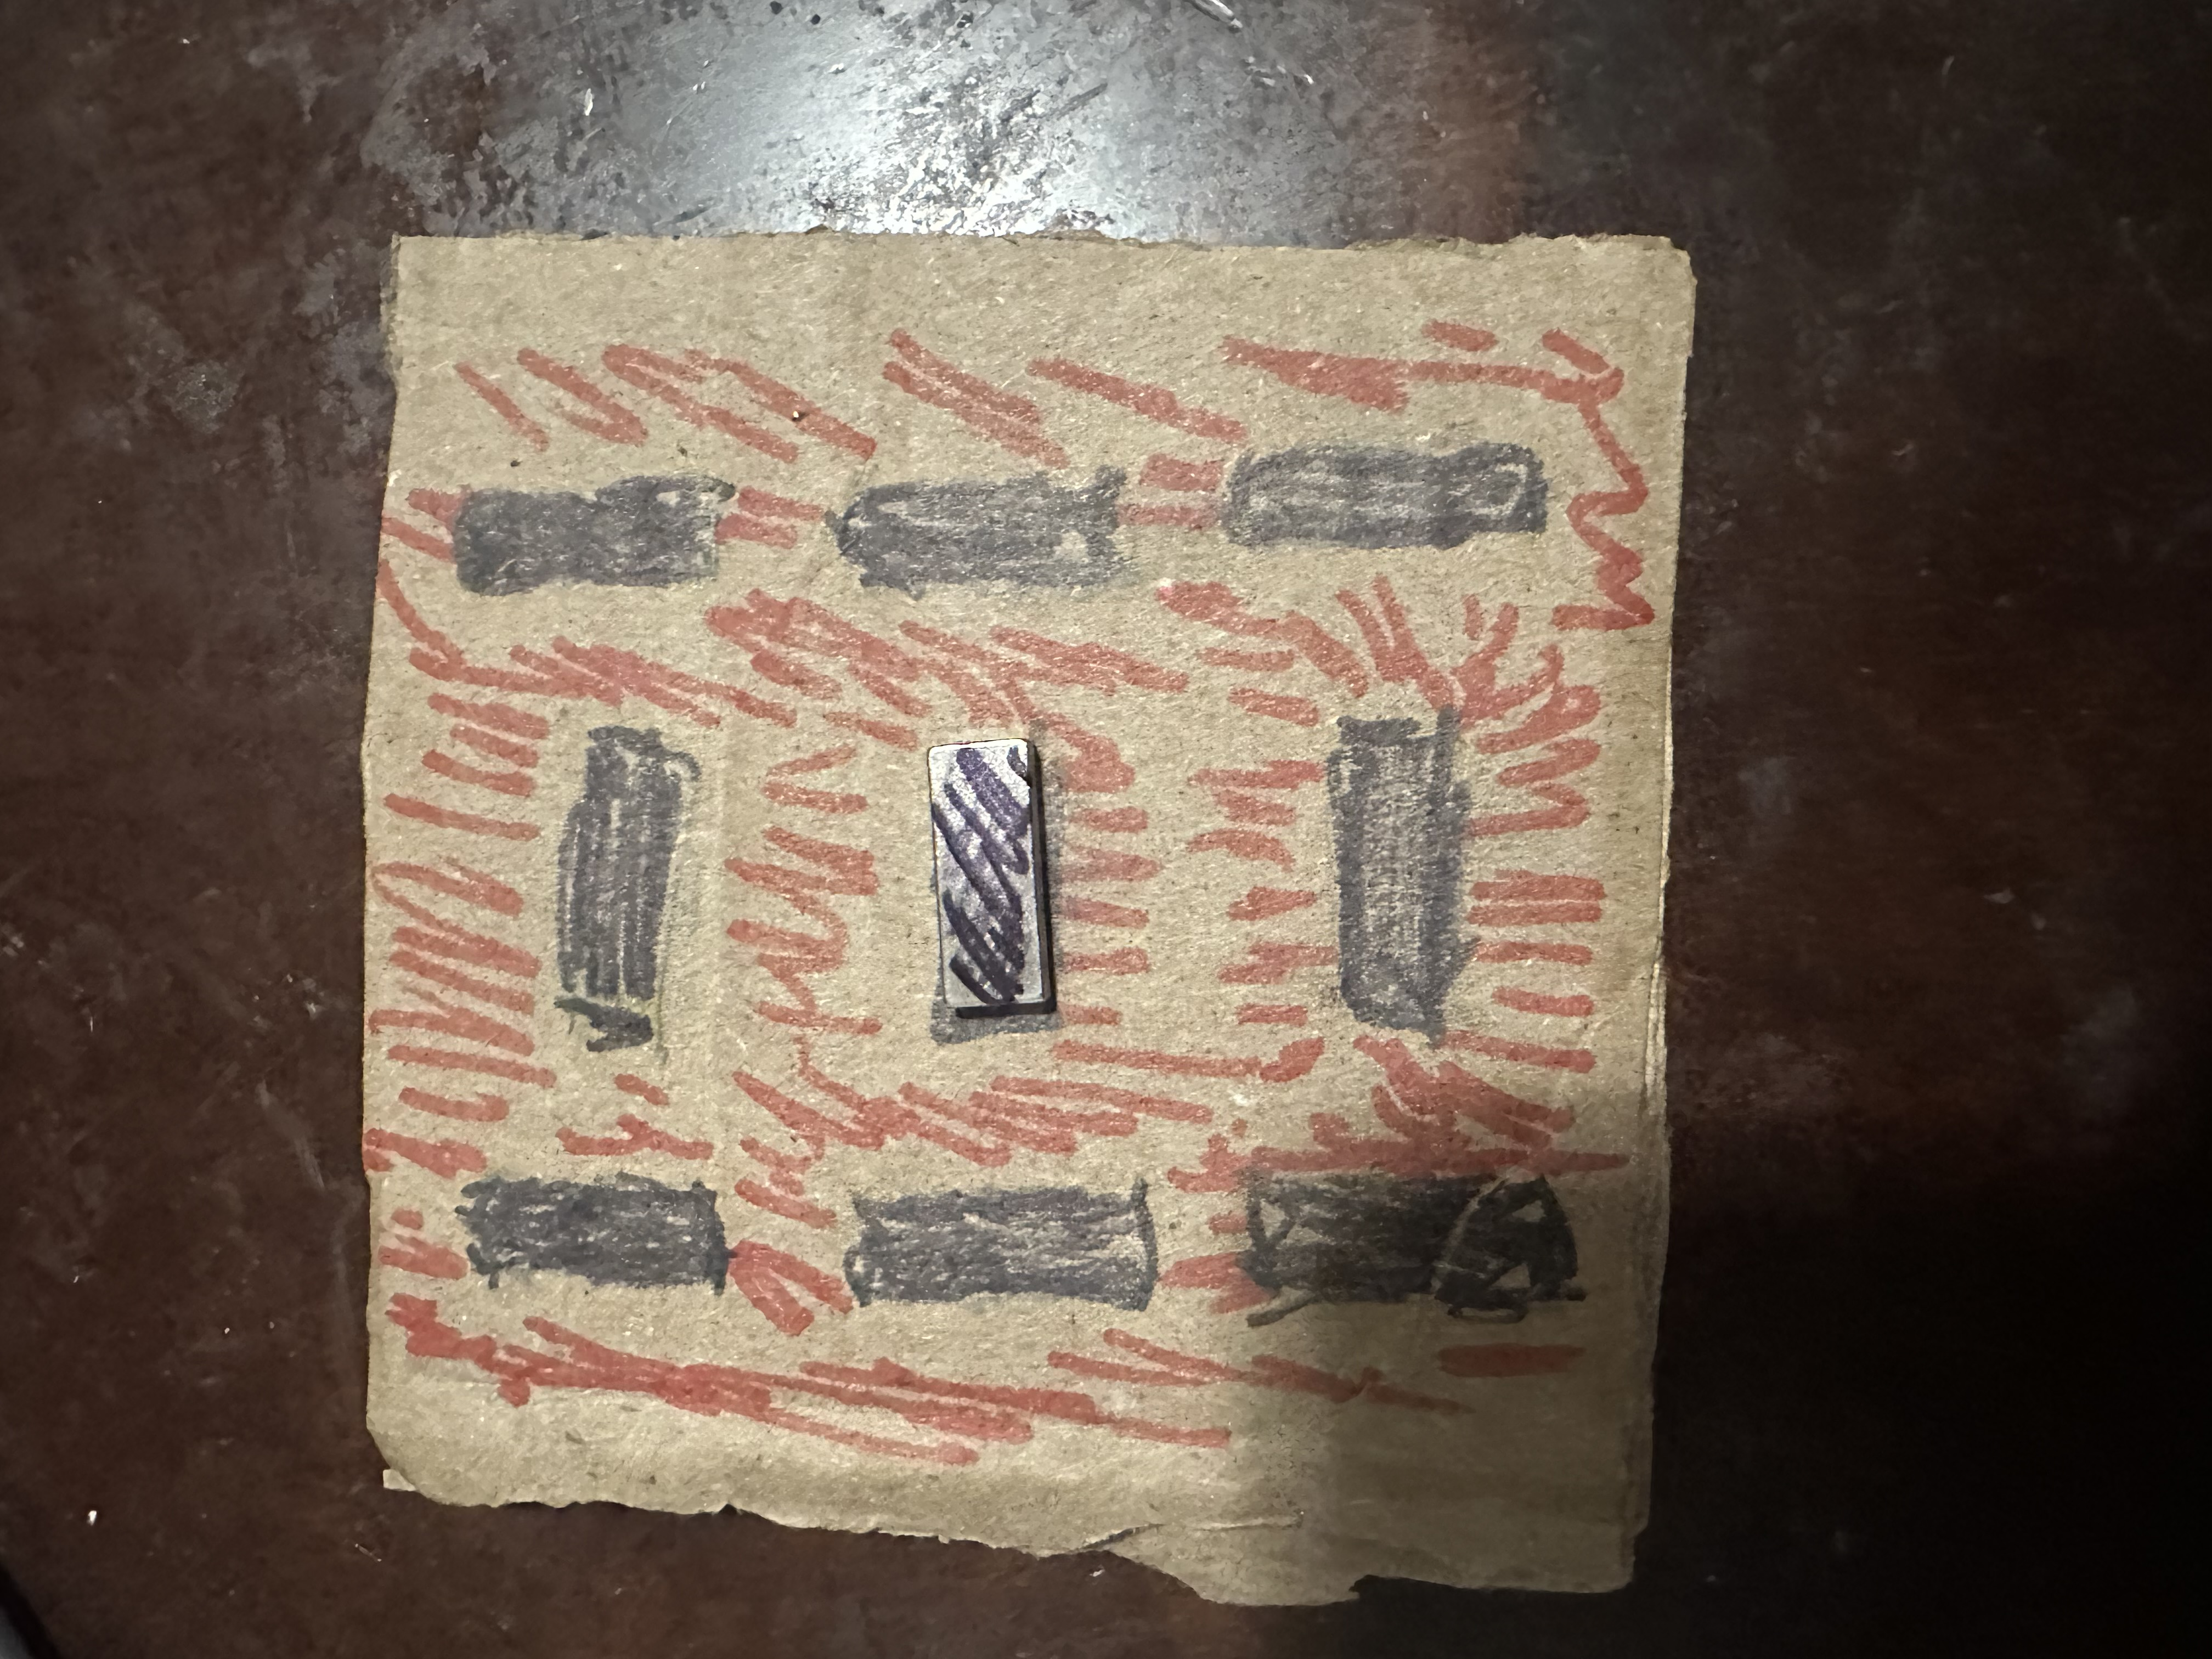
\includegraphics[width=\linewidth]{IMG_0341.jpeg}
    \caption{Field annotated; test magnet at centre.}
  \end{subfigure}\hfill
  \begin{subfigure}{0.31\linewidth}
    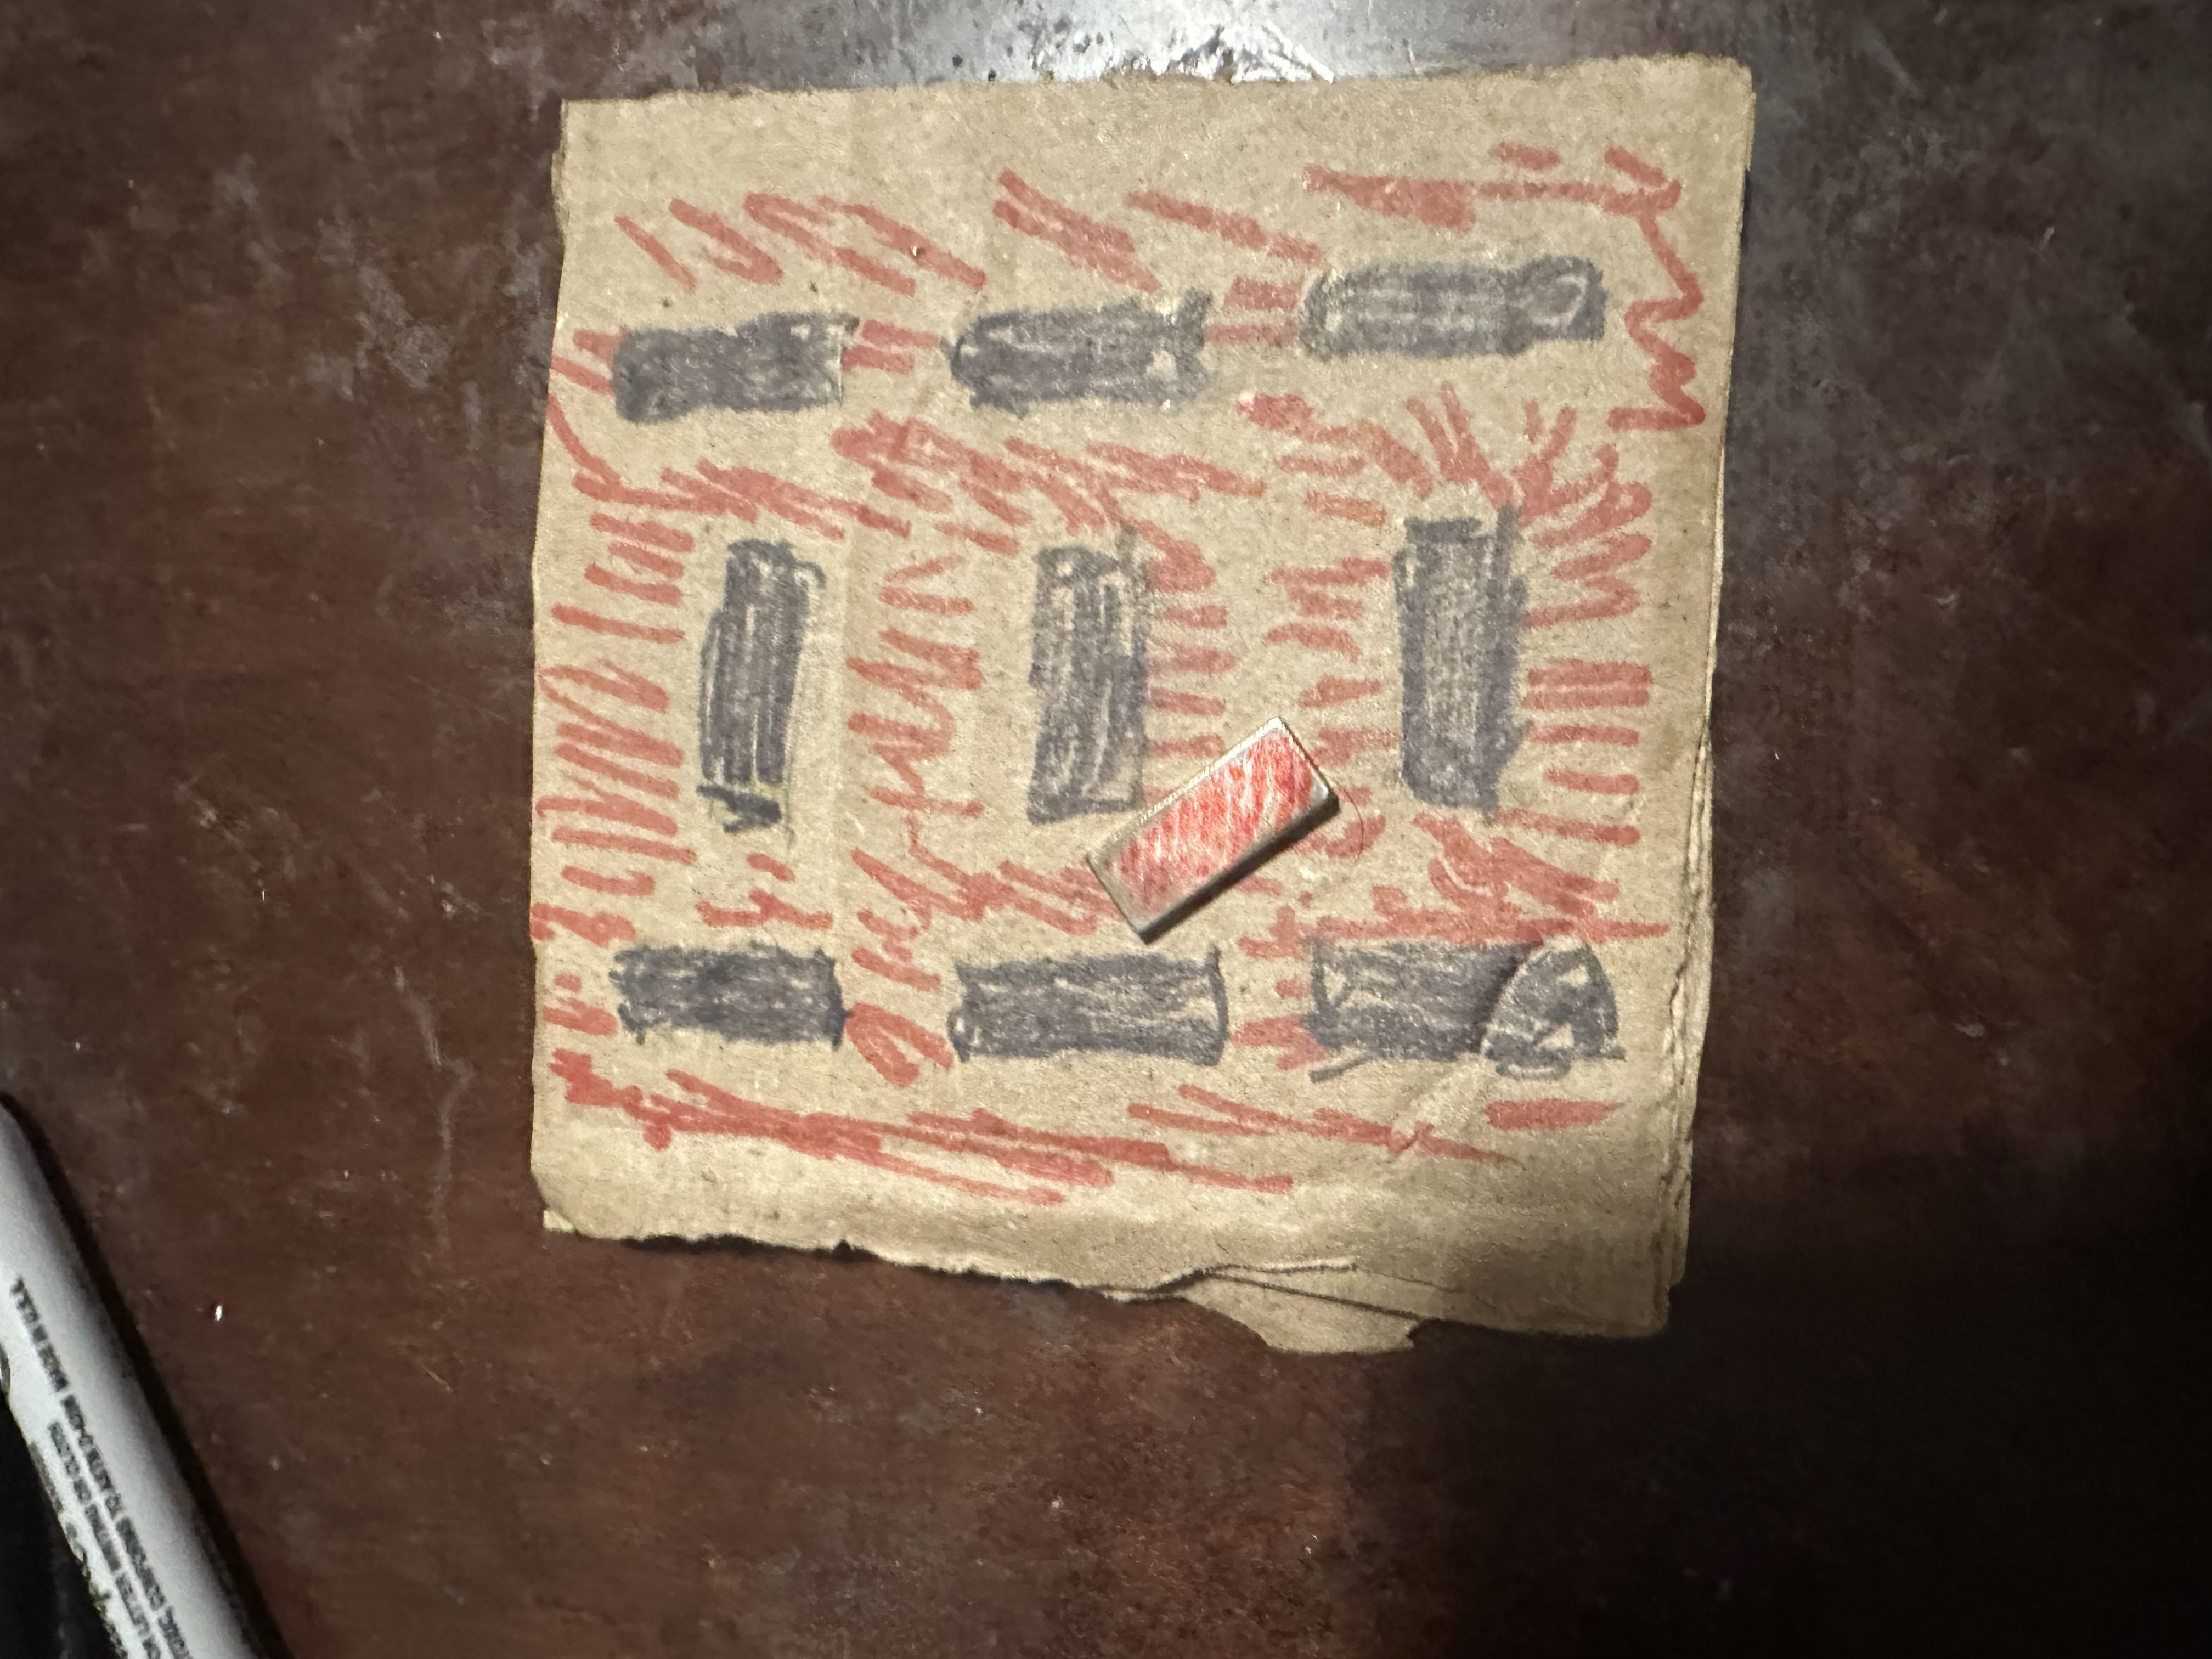
\includegraphics[width=\linewidth]{IMG_0345.jpeg}
    \caption{Polarity / repulsion map.}
  \end{subfigure}
  \caption{Hand planning of the ground-magnet layout on cardboard
  (black = north pole, red = south pole). Although every magnet was placed
  north-up, south poles appear in the gaps between them; the loose magnet is
  moved around to feel out the resulting lift/attraction regions.}
  \label{fig:sketches}
\end{figure}

\subsection{Cardboard prototype with real magnets}

I then taped real neodymium block magnets into the planned ring on cardboard
(Figure~\ref{fig:cardboard-real}) to test the interaction with a real floating
magnet directly.

\begin{figure}[H]
  \centering
  \begin{subfigure}{0.48\linewidth}
    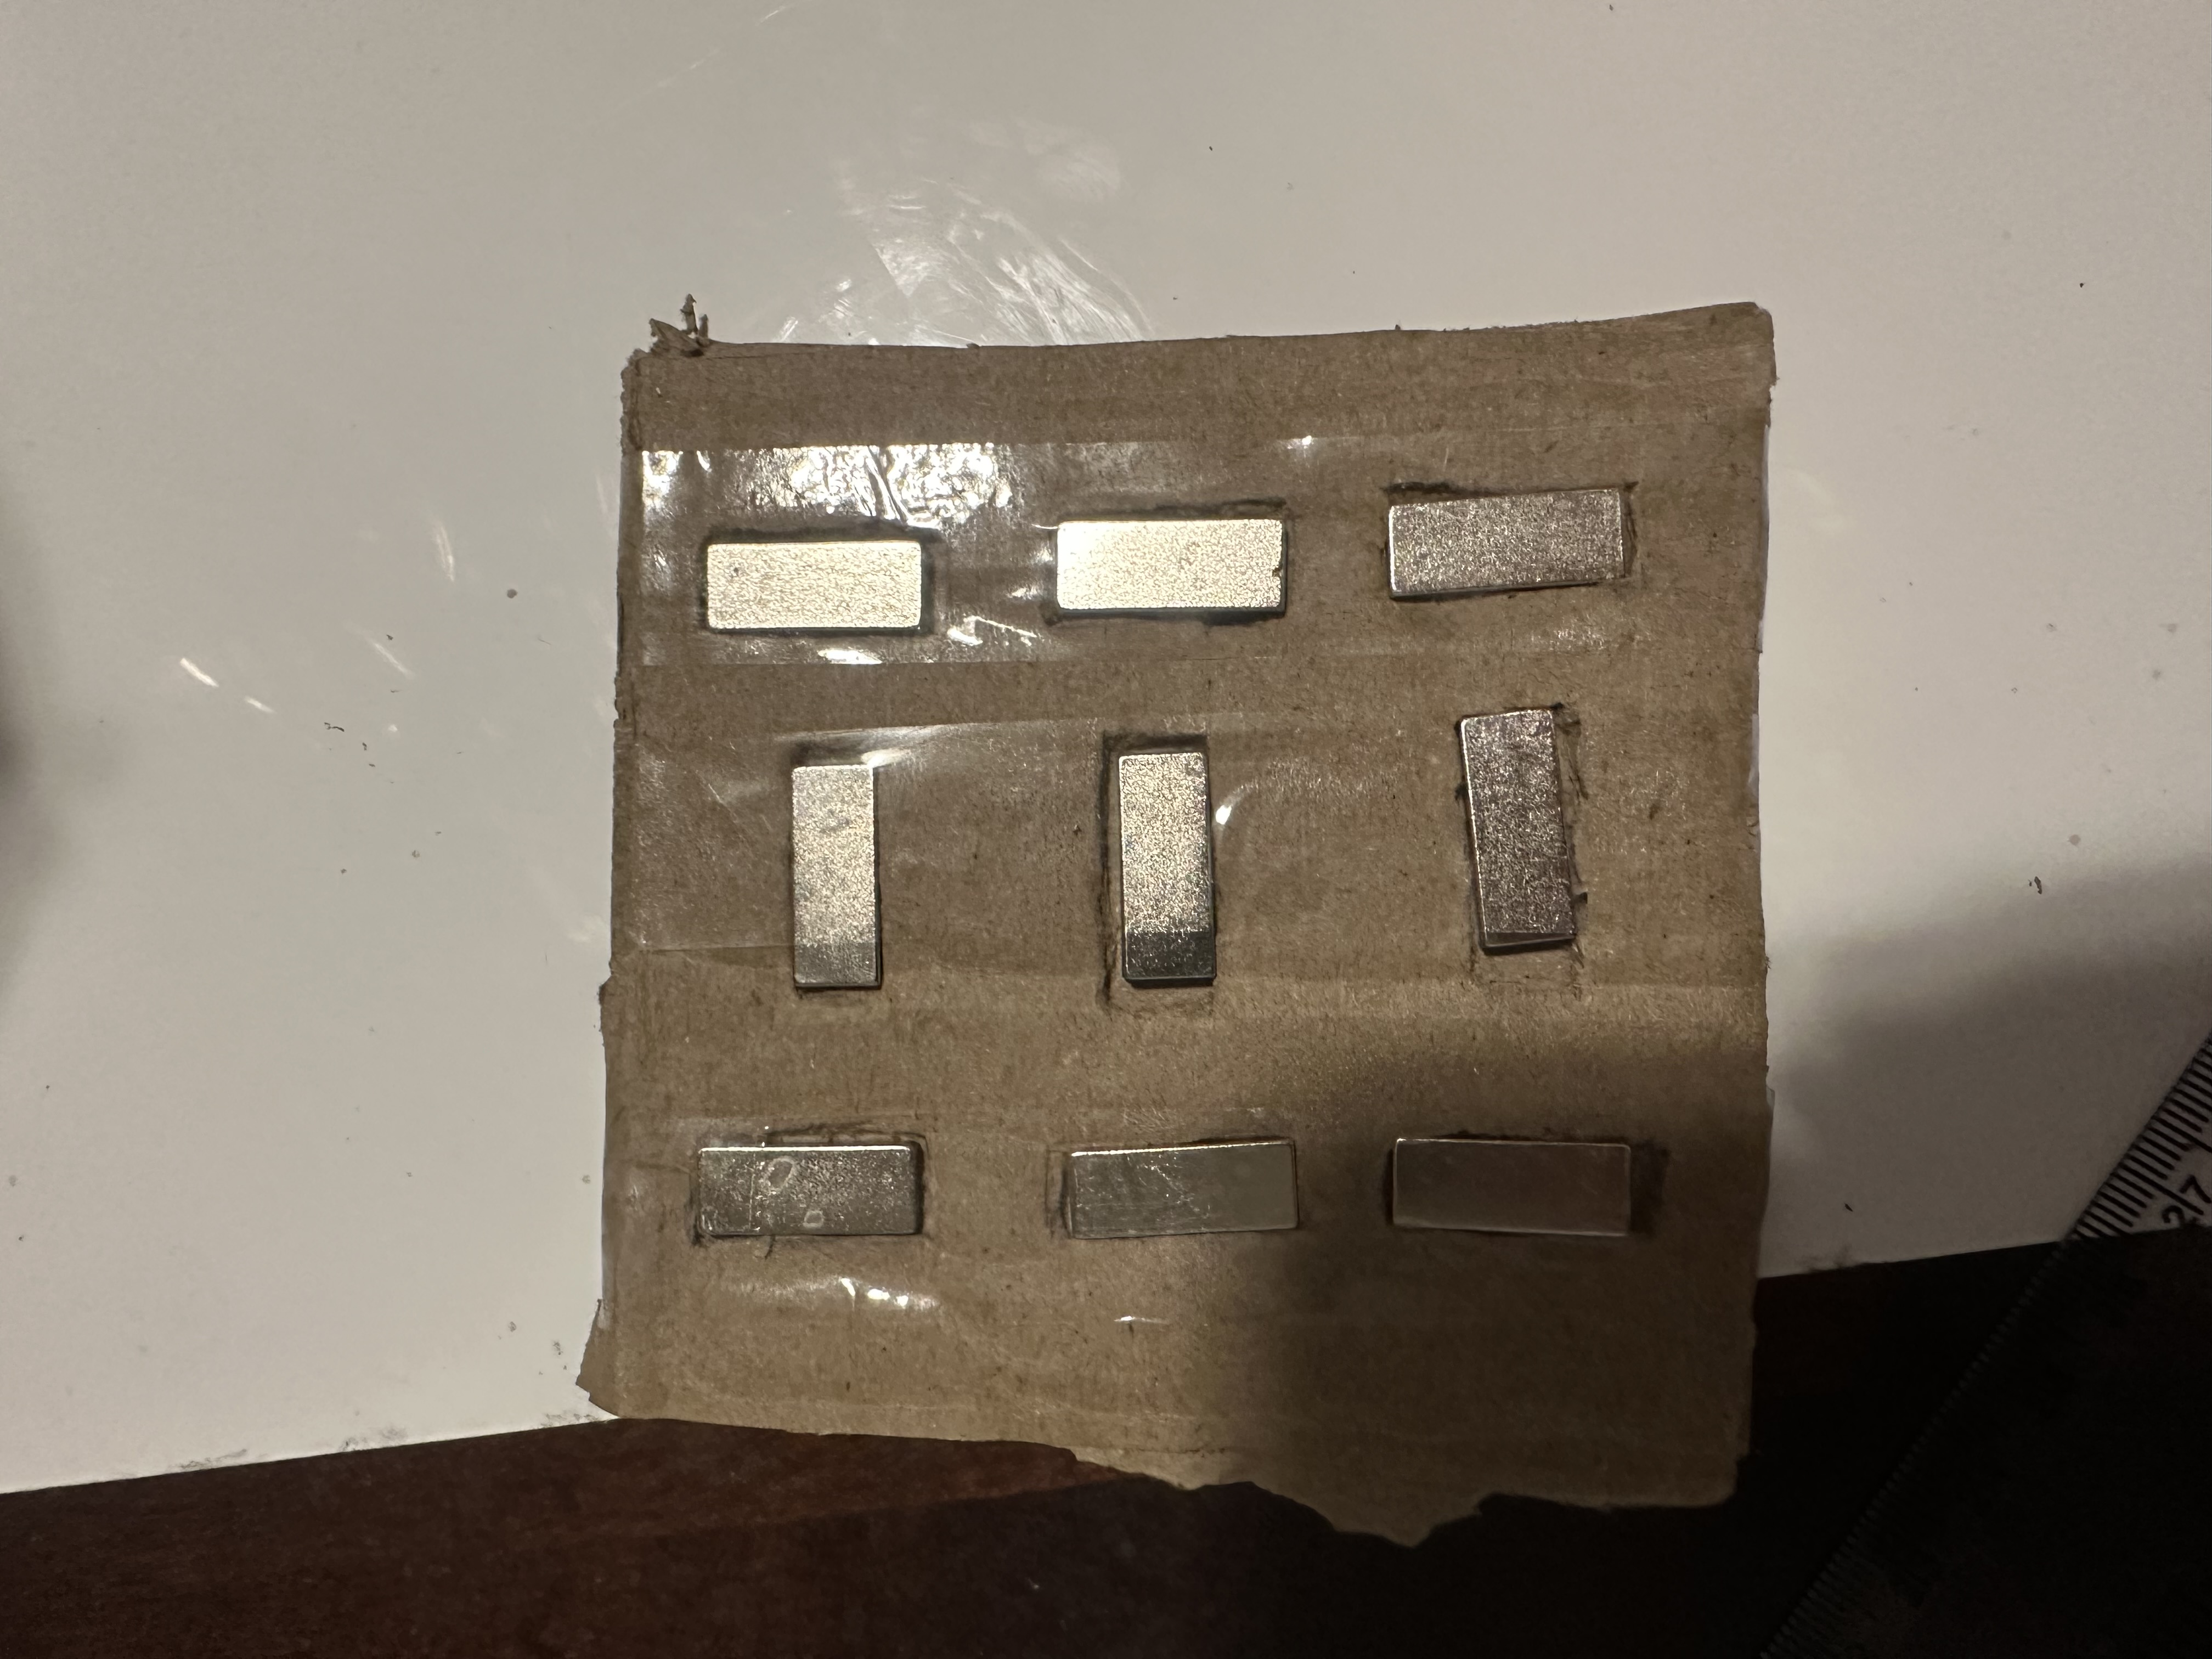
\includegraphics[width=\linewidth]{IMG_0333.jpeg}
    \caption{Real magnets fixed in the planned ring (ruler for scale).}
  \end{subfigure}\hfill
  \begin{subfigure}{0.48\linewidth}
    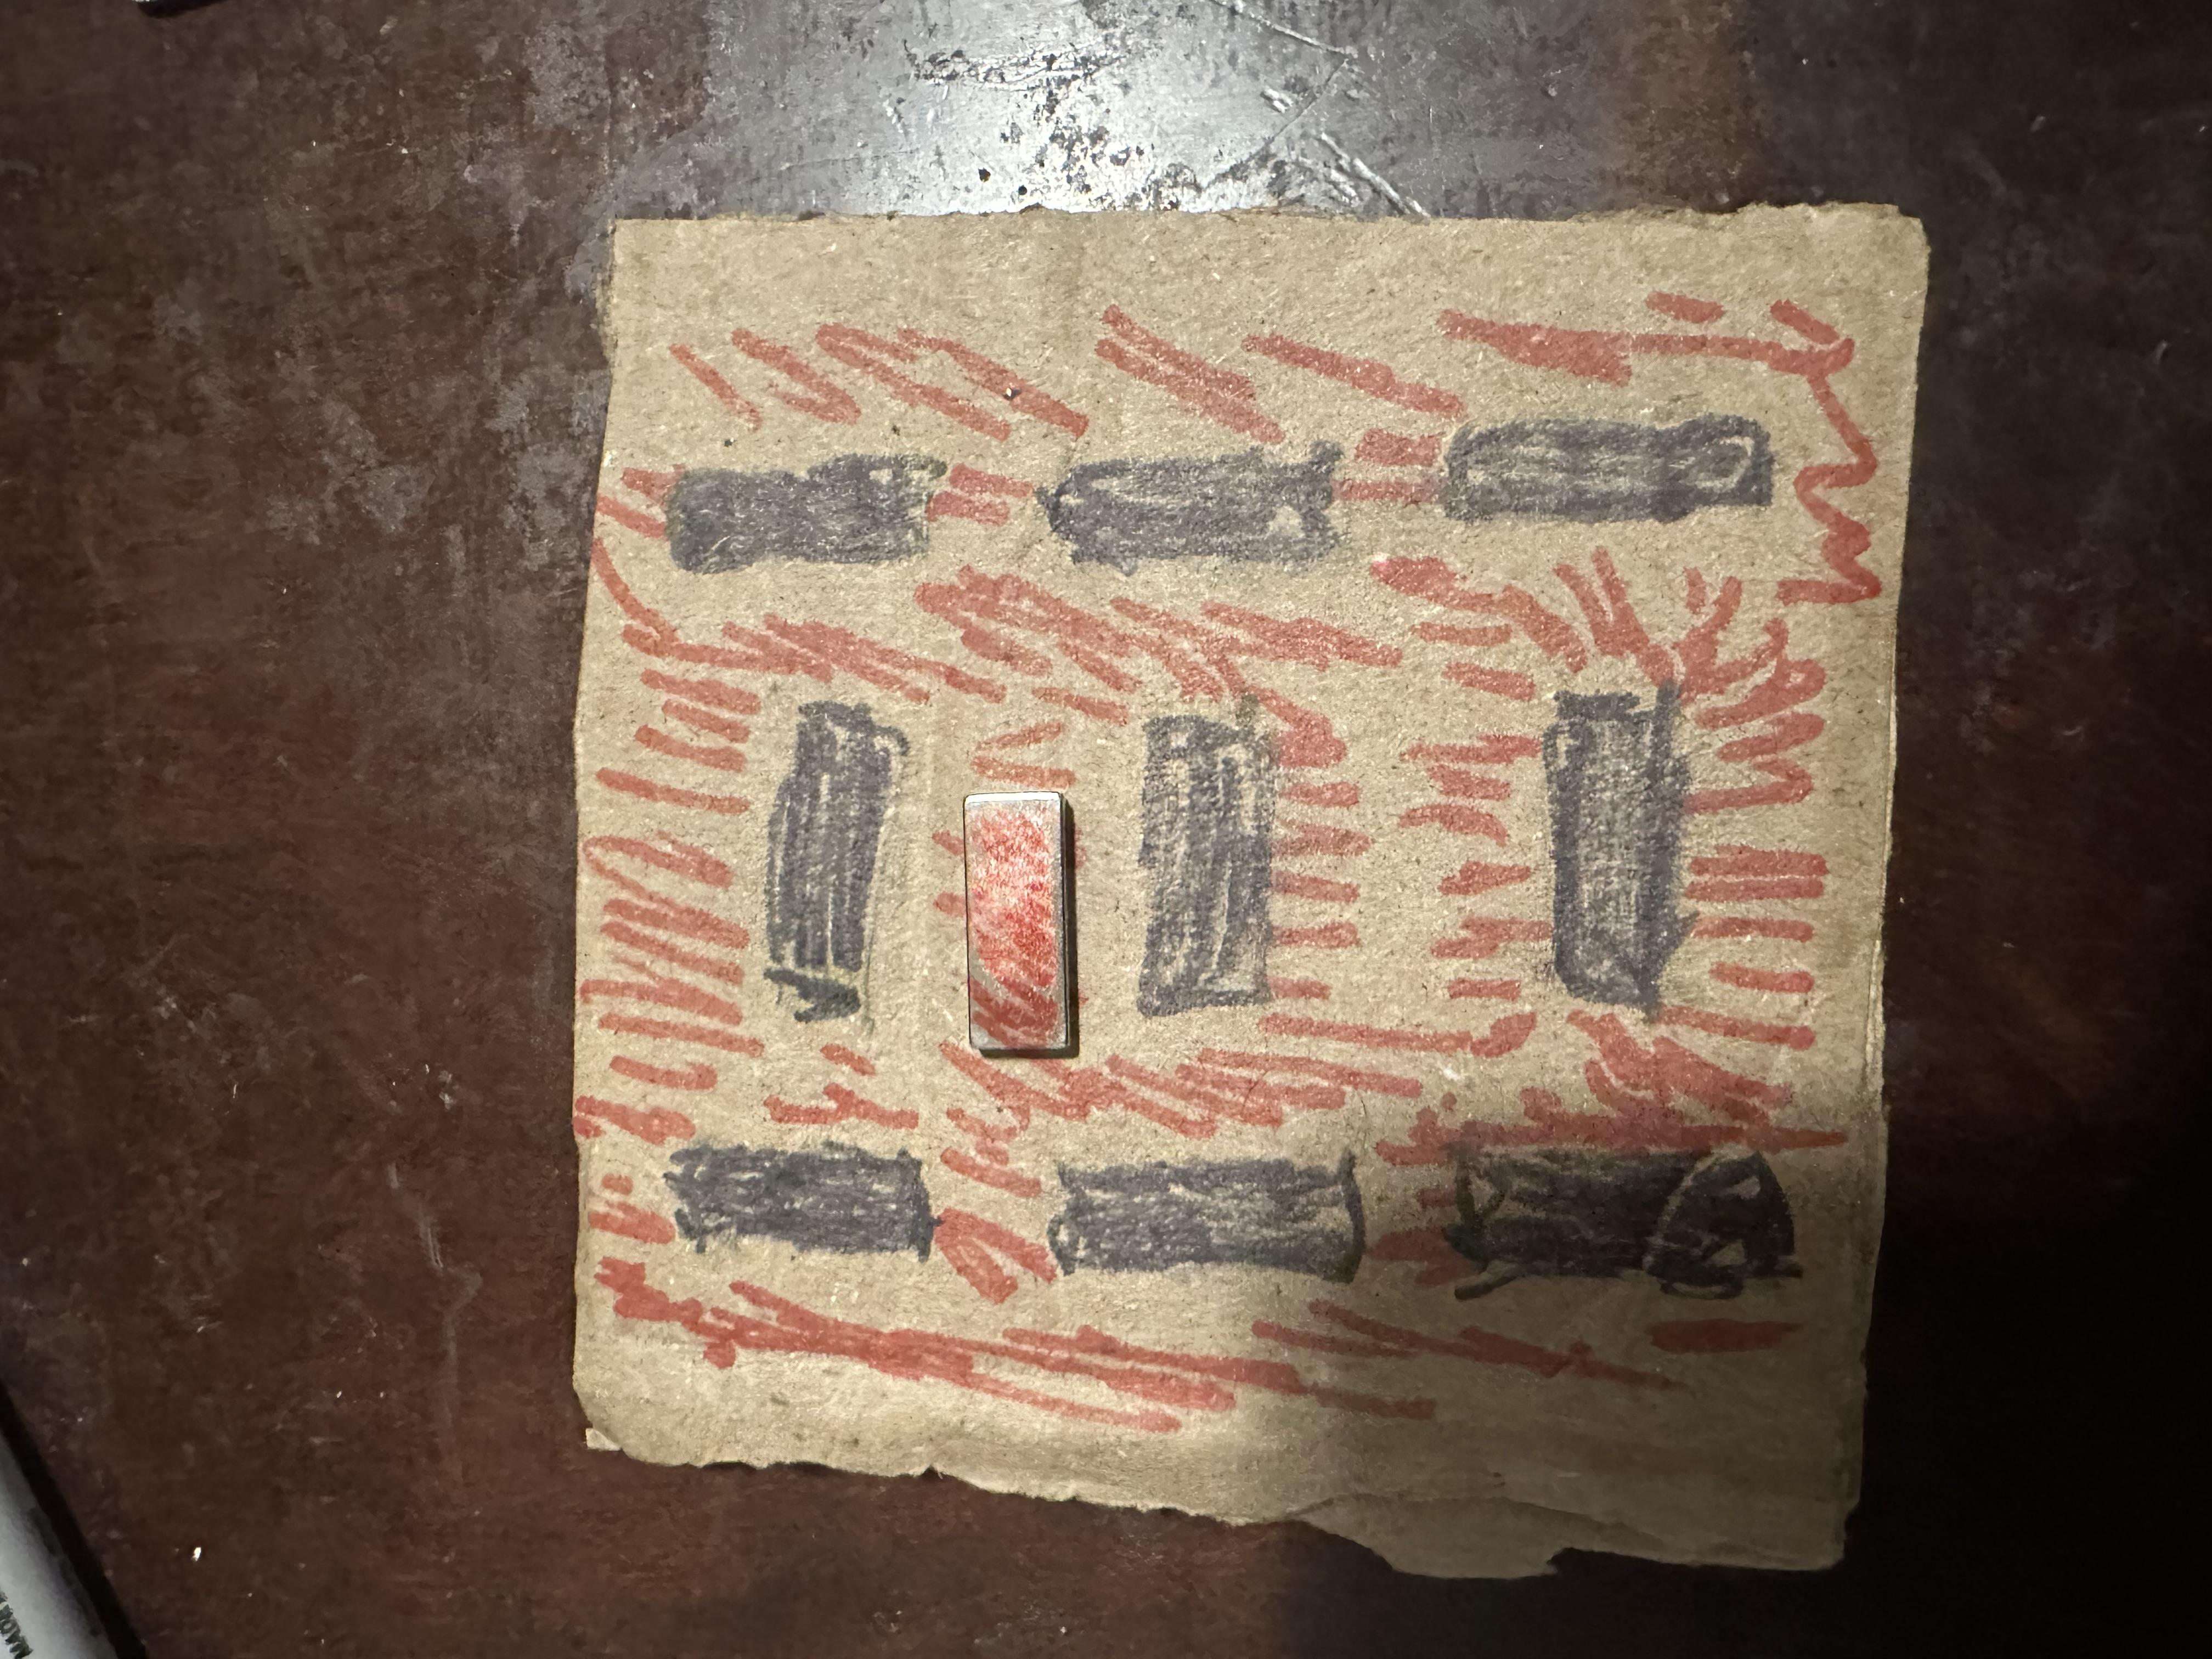
\includegraphics[width=\linewidth]{IMG_0343.jpeg}
    \caption{Layout map with the central test magnet.}
  \end{subfigure}
  \caption{Cardboard prototype of the ground array.}
  \label{fig:cardboard-real}
\end{figure}

\subsection{3-D printed holders}

For a rigid, repeatable build I designed and printed magnet holders (PLA on a
Neptune~3 Pro). The bundle includes both the meshes and the slicer output:
%
\begin{itemize}
  \item \texttt{STLs/magnet\_holder.stl} (+ \texttt{.gcode}) -- the
        \textbf{ground holder}.
  \item \texttt{STLs/levitating\_magnet\_holder.stl} (+ \texttt{.gcode}) -- the
        \textbf{floating platform holder}.
\end{itemize}

The printed holders were a direct response to the cardboard surprise. The cause
of the unwanted attraction was magnets spaced too far apart, letting south poles
appear in the gaps. So this time I packed the magnets \emph{close together}
inside each holder, aiming to suppress those in-between south poles and keep the
field repulsive even between magnets.

I then arranged the holders (all north-up) in a \textbf{triangle}, with a
specific stability idea in mind: the centroid of the triangle is far enough from
all three holders that its repulsion is slightly weaker than directly over any
one of them, but still repulsive. I reasoned that a weaker push in the middle
surrounded by a stronger push at the three corners would form a ``well'' that
traps the floating platform at the centre -- pushing it back inward whenever it
drifted toward a corner.

The final assembly (Figure~\ref{fig:printed}) uses three printed holders joined
by wooden sticks into a triangular frame, each capped with a domed cover holding
several magnets.

\begin{figure}[H]
  \centering
  \begin{subfigure}{0.48\linewidth}
    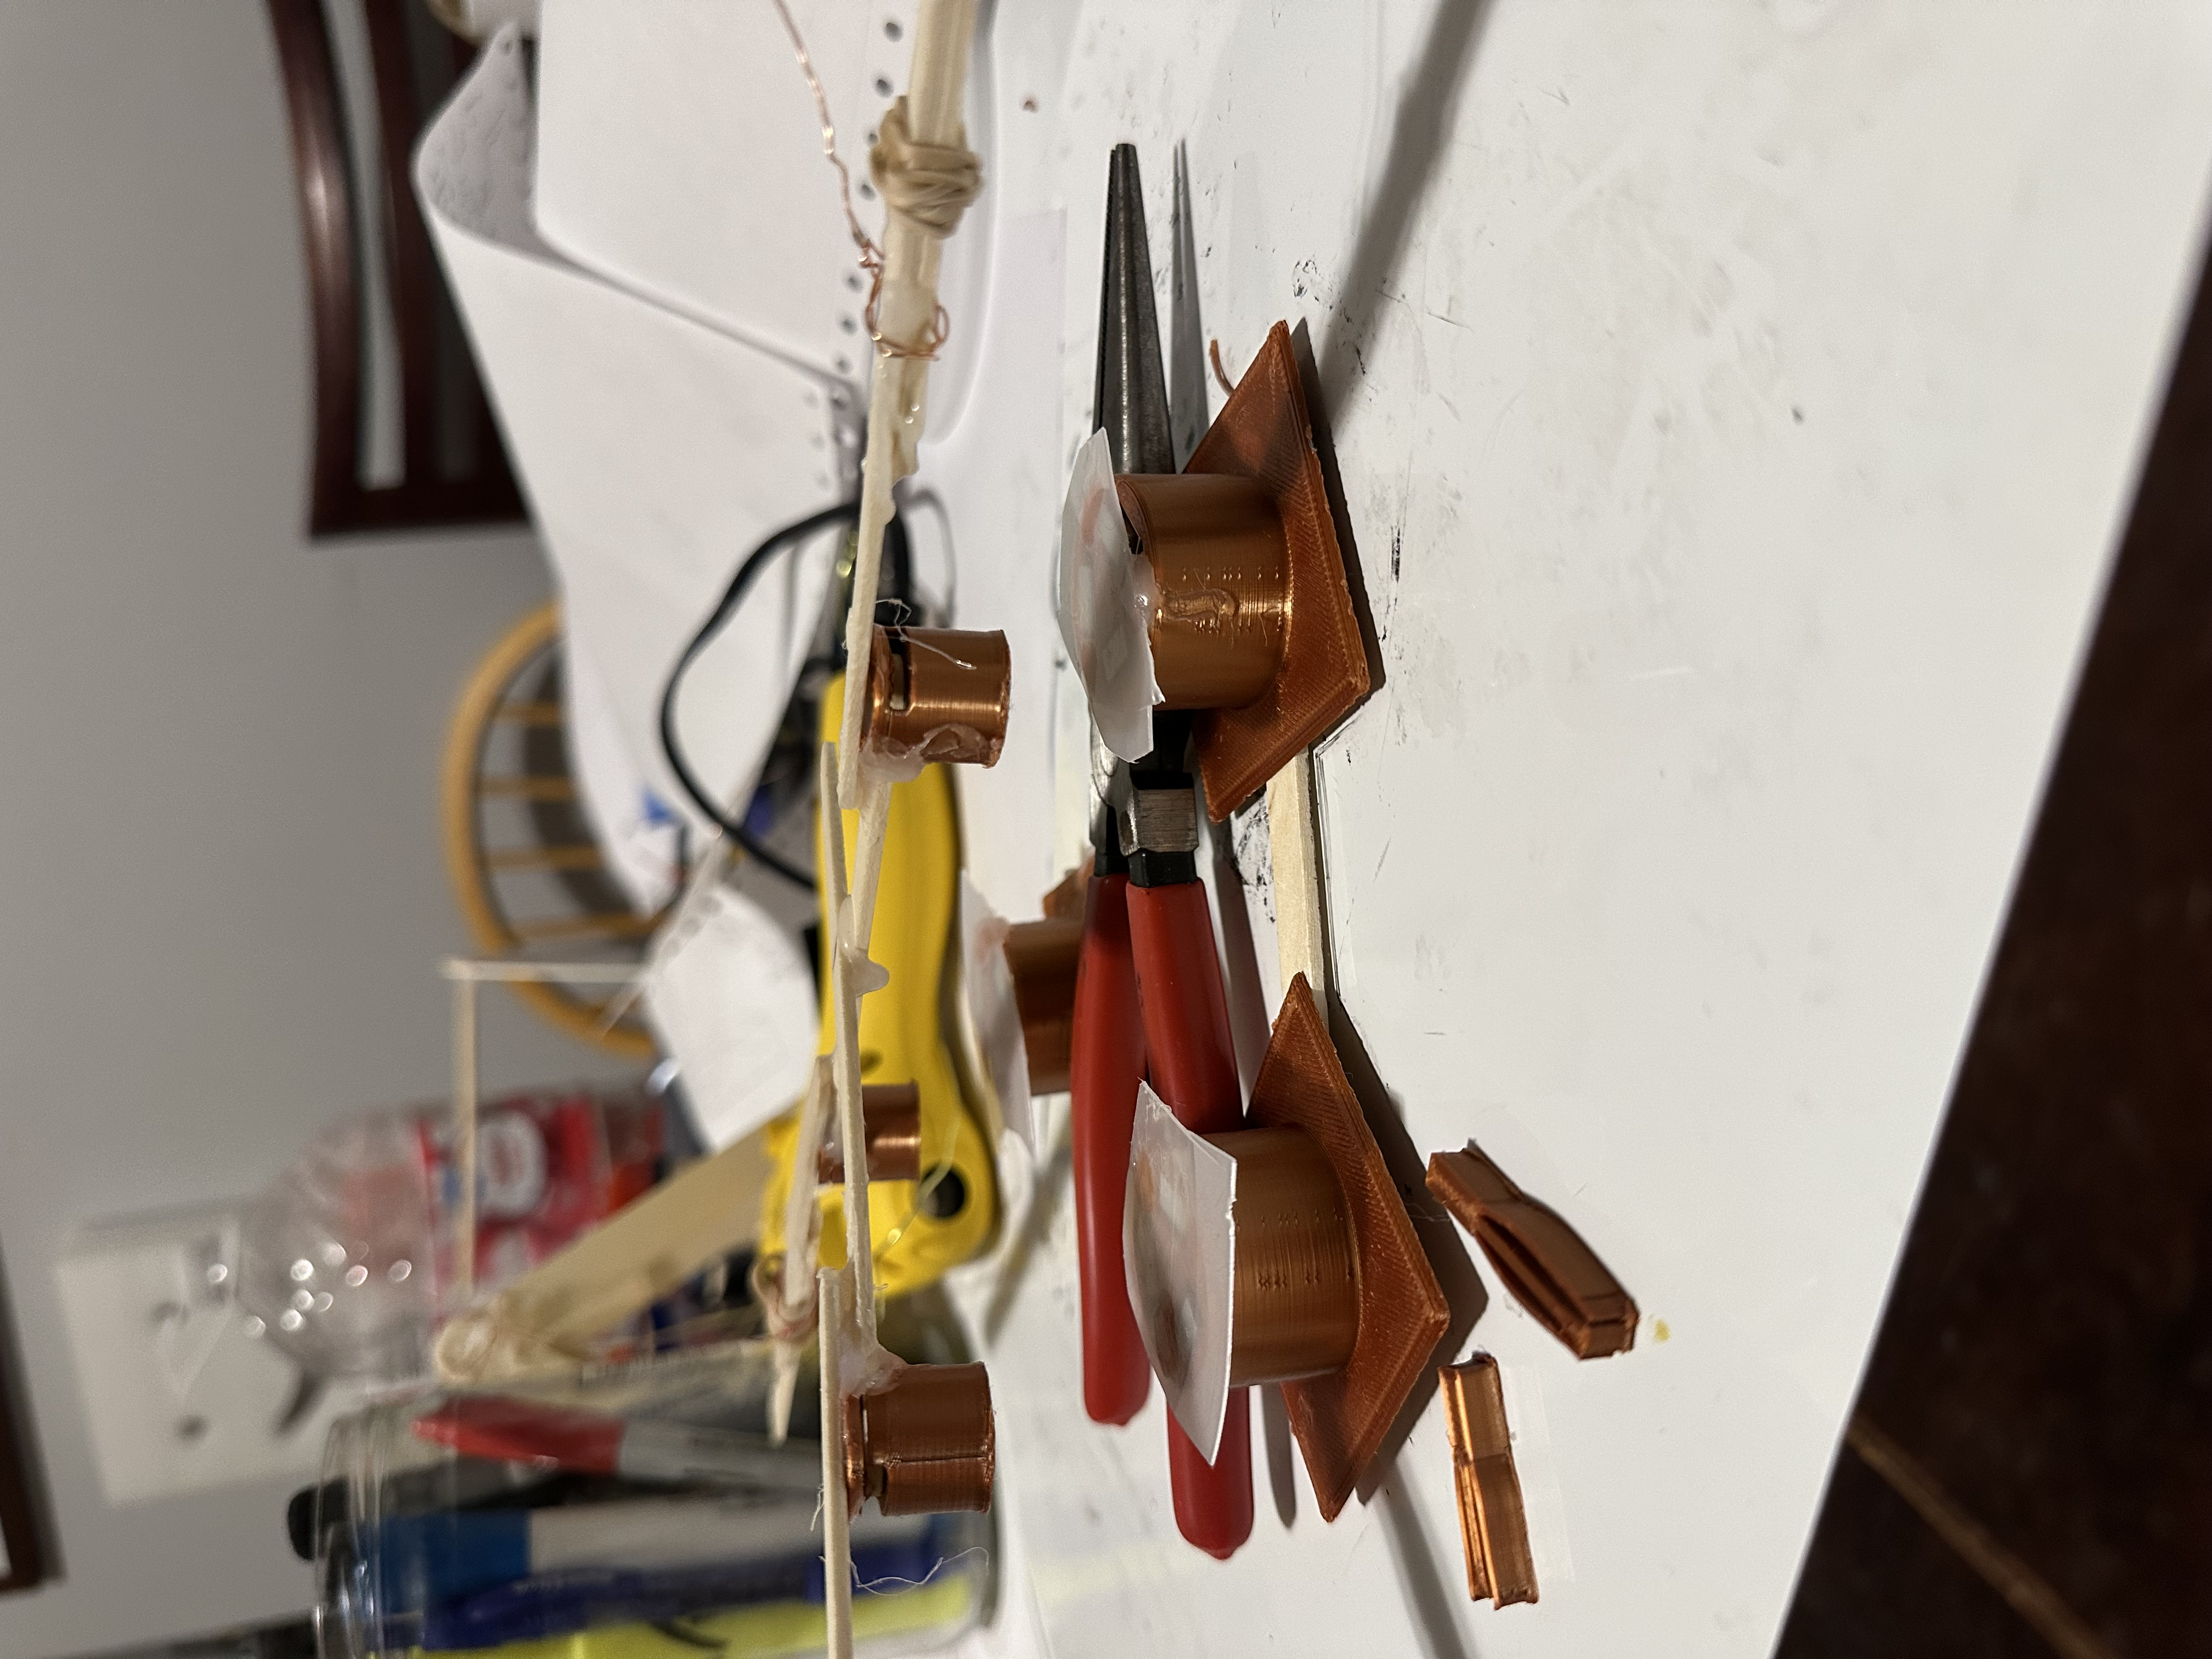
\includegraphics[angle=-90,width=\linewidth]{IMG_0402.jpeg}
    \caption{Printed holders during assembly.}
  \end{subfigure}\hfill
  \begin{subfigure}{0.48\linewidth}
    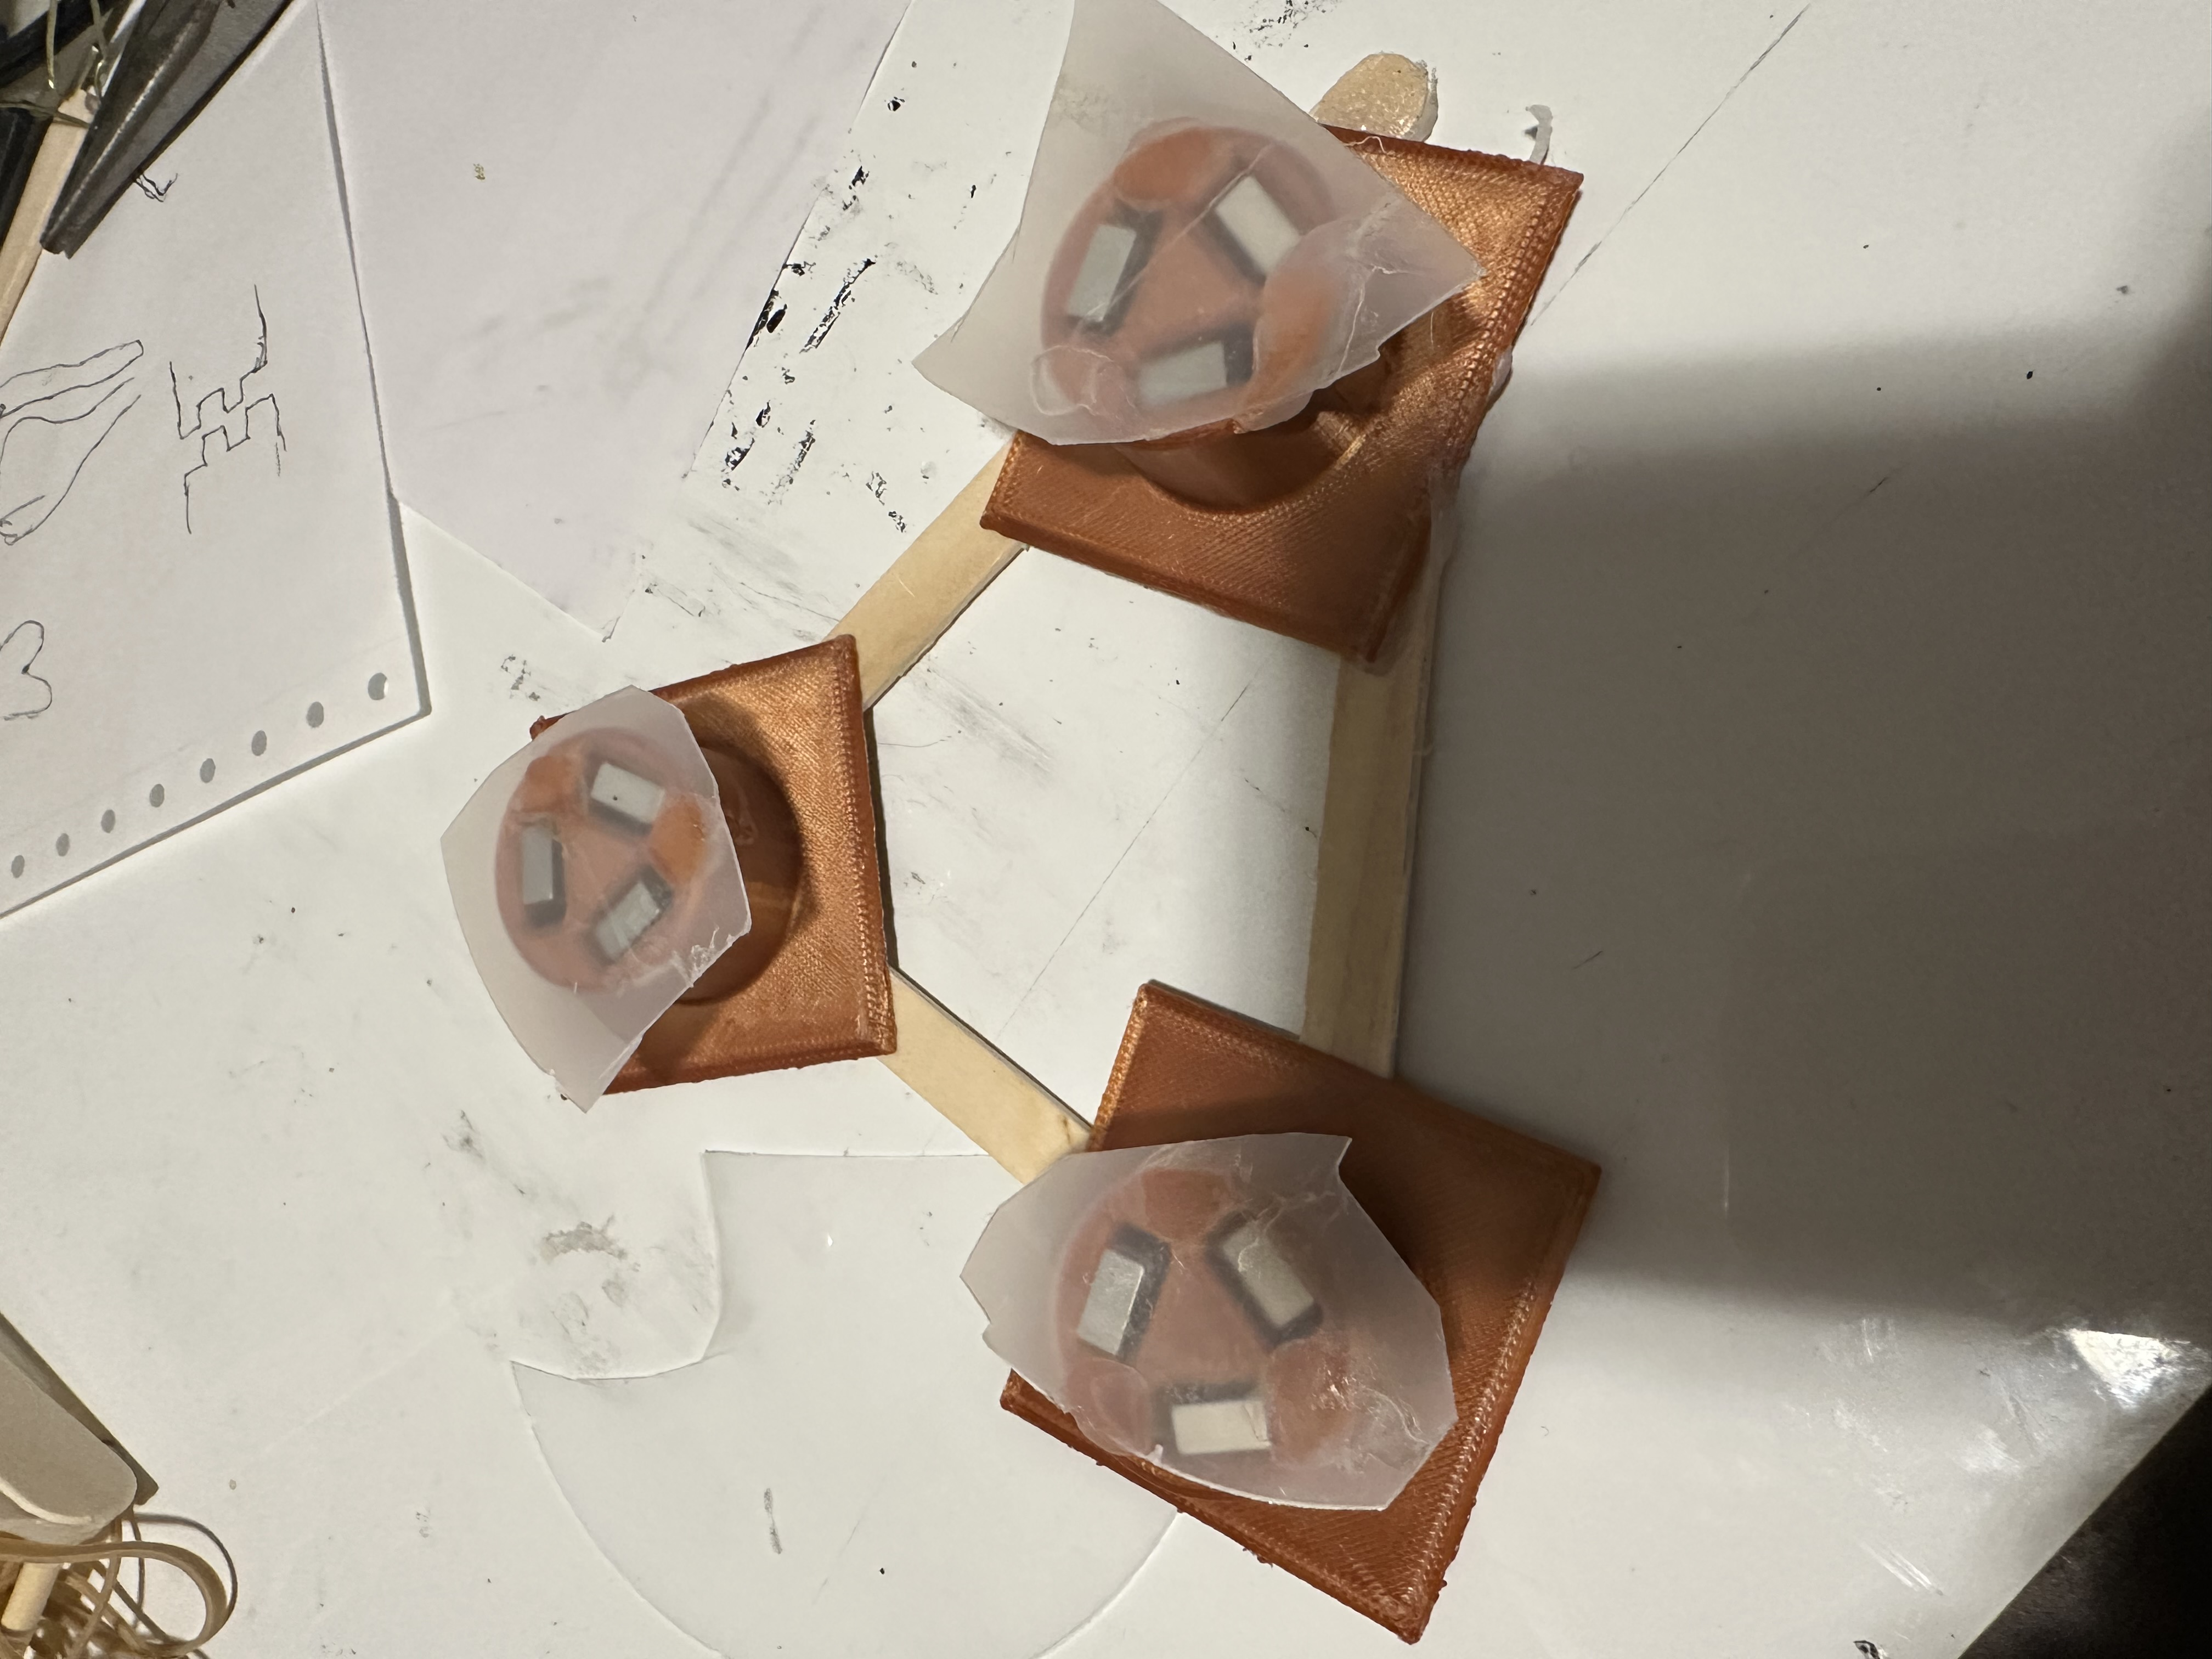
\includegraphics[angle=-90,width=\linewidth]{IMG_0399.jpeg}
    \caption{Triangular frame; three holders, magnets under domed caps.}
  \end{subfigure}
  \caption{3-D printed magnet holders and the assembled triangular frame.}
  \label{fig:printed}
\end{figure}

\subsection{Test and observed behaviour}

The assembled platform was tested over the triangular frame. Free levitation was
never achieved: released on its own, the platform always got out of control --
it slid off and flipped rather than settling at the centre, exactly the Earnshaw
instability of Section~\ref{sec:earnshaw}. The triangular ``well'' idea was not
entirely wrong, though: placed between the three holders the platform clearly
\emph{opposed less} and felt noticeably more stable than over a single holder --
there was a real, if shallow, restoring tendency toward the middle. It simply
was not strong enough to overcome the instability, so the platform still
escaped. The closest I came to a hover was a \emph{tethered} one (recorded in
\texttt{project\_photos/tied\_magnet\_levitation\_video.mp4}), where a tie
removes the runaway horizontal/tilt freedom while the magnets carry the weight.
This matches both predictions: the centre is a slightly more favourable spot
(consistent with the weaker-middle reasoning), but it is still a saddle, not a
true minimum, so without the tether the platform leaves it.

% =============================================================================
\section{Results and discussion}
% =============================================================================

The two failure modes seen on the bench are precisely the two predicted by
theory and reproduced in simulation:
%
\begin{enumerate}
  \item \textbf{It tips and slides (instability).} Earnshaw's theorem
        (Section~\ref{sec:earnshaw}): a static inverse-square equilibrium is at
        best a saddle, never a minimum. Stability in $z$ \emph{forces}
        instability in $x$, $y$, or tilt. The simulation showed it; the bench
        showed it; the tether exists precisely to suppress it.
  \item \textbf{There is barely any net lift (weakness).} The plane-cancellation
        of Section~\ref{sec:lineplane}: averaged over a flat platform's area,
        the vertical force tends to zero because $\nabla\cdot\mathbf{B}=0$. The
        optimizer's diagnostics (Figure~\ref{fig:diagnosis}) show the net force
        hovering near zero with a negative tail, no matter the layout.
\end{enumerate}
%
Together these explain why the intuitive ``magnets repel, so a platform should
float'' picture fails: the lift is both \emph{unstable} and \emph{weak}, and the
two problems get worse, not better, as you scale the platform up.

% =============================================================================
\section{Conclusion}
% =============================================================================

The platform did not float freely, and it could not have: a static array of
permanent magnets cannot hold a body in stable levitation (Earnshaw), and a flat
platform barely develops any net lift because the vertical force cancels when
averaged over a plane (no magnetic monopoles). The simulation, hand-drawn field
maps, cardboard prototype, and 3-D printed build all converge on the same
conclusion, and -- usefully -- the optimizer turned a vague ``the force seems
too small'' into a quantitative, explained result. The deliverable is therefore
not a levitating platform but a clear, evidence-backed account of why
permanent-magnet levitation is hard.

% =============================================================================
\appendix
\section{File manifest}
% =============================================================================

\sloppy
\begin{itemize}
  \item \texttt{graphs/} -- force-field figures and the scripts that generate
        them; see \texttt{graphs/description\_of\_graphs.md}.
  \item \texttt{Attempt\_3/} -- single-magnet force field
        (\texttt{magnet\_strength.py}) and the layout optimizer
        (\texttt{platform\_optimizer/optimizer.py}), with diagnostics
        \texttt{diagnosis.png}, \texttt{line\_vs\_plane.png}.
  \item \texttt{STLs/} -- printable meshes and sliced \texttt{.gcode} for the
        magnet holders.
  \item \texttt{designs/} -- the layout design canvas.
  \item \texttt{project\_photos/} -- build photos and the tethered-hover video.
\end{itemize}

\end{document}
